\documentclass[10.5pt,a4paper]{article}
\usepackage[margin=2.1cm]{geometry}
\usepackage{amsmath,amssymb}
\usepackage[table]{xcolor}
\usepackage{booktabs,tabularx,array}
\usepackage{enumitem}
\usepackage{graphicx}
\usepackage[most]{tcolorbox}
\usepackage[hidelinks]{hyperref}
\hypersetup{pdftitle={Protocol suggestions for xyz}}
\usepackage{titlesec}
\usepackage{needspace,etoolbox,xltabular}
\pretocmd{\section}{\needspace{8\baselineskip}}{}{}
\pretocmd{\subsection}{\needspace{6\baselineskip}}{}{}
\titlespacing*{\subsection}{0pt}{1.1ex plus .3ex}{.5ex}
\setlength{\parindent}{0pt}
\setlength{\parskip}{.35ex}

% changed terms: blue text (the charts' proposal blue); removed terms: red
\definecolor{chg}{RGB}{255,214,153}
\definecolor{rem}{RGB}{200,40,40}
\definecolor{lead}{RGB}{20,120,60}
\definecolor{rej}{RGB}{170,40,40}
\definecolor{sup}{RGB}{110,110,110}
\definecolor{pend}{RGB}{30,90,170}
\newcommand{\chg}[1]{\ensuremath{{\color[HTML]{2F74D0}#1}}}
\newcommand{\rem}[1]{\textcolor{rem}{\ensuremath{#1}}}
\newcommand{\med}{\operatorname{med}}
\newcommand{\clip}{\operatorname{clip}}
\newcommand{\vwmed}{\operatorname{vwmed}}
\newcommand{\ema}{\operatorname{EMA}}
\newcommand{\D}{\mathcal{D}}
% status line: \st{colour}{status}{who ships it}
\newcommand{\st}[3]{\textcolor{#1}{\textbf{#2}} \,·\, \emph{#3}\par}
\newcommand{\res}[1]{\par\textbf{What the replay showed.} #1\par}
\newcommand{\resh}[2]{\par\textbf{#1} #2\par}

% --- core pages (paper_core.tex): one idea per page
\definecolor{today}{HTML}{E8683A}
\definecolor{vault}{HTML}{1FAF7A}
\definecolor{mute}{HTML}{6B6B6B}
\definecolor{rule}{HTML}{E9E7E2}
\definecolor{boxbg}{HTML}{F7F6F3}
% core formulas page: a term that differs from today's rules, in the charts' proposal blue
\definecolor{prop}{HTML}{2F74D0}
\newcommand{\nw}[1]{{\color{prop}#1}}
% today vs proposal, at the top of each change page
\newcommand{\changerule}[2]{{\small\renewcommand{\arraystretch}{1.3}\setlength{\tabcolsep}{5pt}%
\noindent\begin{tabularx}{\textwidth}{@{}>{\bfseries\raggedright\arraybackslash}p{1.75cm}>{\raggedright\arraybackslash}X@{}}\toprule
\textcolor{today}{Today} & #1\\ \textcolor{prop}{Suggested} & #2\\\bottomrule\end{tabularx}}\par\vspace{.6ex}}
% \page{message title}{tag line}: starts a new page
\newcommand{\page}[2]{\clearpage{\LARGE\bfseries\raggedright #1\par}\vspace{.3ex}{\parskip=0pt\color{mute}\small #2\par}\vspace{1.2ex}}
\newcommand{\foot}{\par\vspace{1.5ex plus 1fil}}
% the technical block at the foot of a core page
\newtcolorbox{exact}[1][The rule, exactly]{enhanced,colback=boxbg,colframe=rule,boxrule=.5pt,arc=1.5pt,left=7pt,right=7pt,top=5pt,bottom=5pt,
  fonttitle=\bfseries\small,coltitle=black,colbacktitle=boxbg,title={#1},fontupper=\small}
\newtcolorbox{words}[1][Words used]{enhanced,colback=white,colframe=rule,boxrule=.5pt,arc=1.5pt,left=7pt,right=7pt,top=5pt,bottom=5pt,
  fonttitle=\bfseries\small,coltitle=black,colbacktitle=white,title={#1},fontupper=\small}
\newcommand{\ptag}[2]{\textcolor{#1}{\textbf{#2}}}
% a chart that sim/figs.py does not draw yet
\newcommand{\chartpending}[1]{\begin{center}\fcolorbox{rule}{white}{\parbox[c][6.2cm][c]{.95\textwidth}{\centering\color{mute}\small\emph{Chart to come:} #1}}\end{center}}

\begin{document}
% core pages: larger type, and spare height shared between paragraphs so no page ends half empty
{\fontsize{11.5pt}{15.5pt}\selectfont\setlength{\parskip}{1ex plus .35fil}
% Core of mark_formulas.tex: one idea per page, written for a reader who has never seen the study.
% Pages: summary, problems, one page per change, how they fit, the formulas side by side; then the tests and what they showed; costs; limits.
% Numbers: docs/results/scorecard.md (final run of 2026-11-11) unless a page's box says otherwise.

%======================================================================================== 1 summary
\begin{center}
{\LARGE\bfseries Protocol suggestions for xyz\par}
\vspace{.5ex}
{\normalsize\bfseries Changes trade.xyz and Hyperliquid could consider for stressed markets\par}
\vspace{.9ex}
{\large @ymsynn\par}
{\small\texttt{ymsynnquant@gmail.com} \,·\, November 13, 2026\par}
{\small Rule explorer: \href{https://ymsynn.github.io/xyz-backstop-study/}{\texttt{ymsynn.github.io/xyz-backstop-study}} \,·\, code and data: \href{https://github.com/ymsynn/xyz-backstop-study}{\texttt{github.com/ymsynn/xyz-backstop-study}}\par}
\end{center}
\vspace{-1ex}

For every HIP-3 deployer, a position the order book cannot close goes to a backstop vault if the market allows cross margin; when it does not, or when the vault cannot take the position, profitable traders are closed out (ADL). On trade.xyz's markets, ADL closed \$85.2M of positions in 392 days. This paper suggests six changes to reduce potential ADL and improve how the backstop vault performs. The main one is the mark price (changes 1 and 2): two changes to what trade.xyz's \emph{relayer} (its price program) publishes, which could be computed beside production.

\begin{center}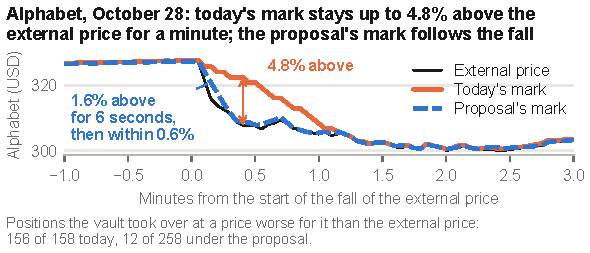
\includegraphics[width=.6\textwidth]{figs/headline_crash.pdf}\end{center}

\vspace{.6ex}
{\small
\begin{tabularx}{\textwidth}{@{}r>{\raggedright\arraybackslash}X>{\raggedright\arraybackslash}p{3.1cm}>{\raggedright\arraybackslash}p{2.6cm}@{}}
\toprule
 & Suggestion & Who would ship it & Serves\\
\midrule
1 & \textbf{Mark price.} Median of the external price, xyz's book and the anchor; a 30-second 5\% wrong price moved it 4.17\% today, 0.10\% & trade.xyz & \ptag{today}{ADL}, \ptag{today}{backstop loss}, \ptag{mute}{attacks}\\
2 & \textbf{Closed market or quiet feed.} One capped rule, under which a short push moves the price slowly & trade.xyz & \ptag{mute}{attacks}\\
\midrule
3 & \textbf{Liquidation size.} With the new mark, cut a large position back to initial margin at once & Hyperliquid & \ptag{today}{backstop loss}\\
4 & \textbf{Vault coverage.} Allow the vault in six more liquid markets & trade.xyz, with validator review & \ptag{today}{ADL}\\
5 & \textbf{Vault capital floor.} A floor recomputed each morning from open positions & trade.xyz & \ptag{vault}{capital}\\
6 & \textbf{External price.} Publish its age and sources; check overnight moves & trade.xyz & \ptag{mute}{attacks}\\
\bottomrule
\end{tabularx}}

\textbf{What the tests show.} We replayed about 85 recorded \emph{market-days} under today's rules and under changes 1 to 3 together (\emph{the proposal}). ADL on five isolated-only markets falls (\$300.4k today, \$99.5k). In most tests the vault inherits more, but on the three earnings crashes together it needs less money to avoid ADL (\$462k, \$352k) and less capital (\$715k, \$589k); on Alphabet alone, more. The cut-back (3) helps only with the new mark (page~\pageref{sec:res-cut}). Costs: page~\pageref{sec:costs}.

\foot
\begin{words}
\begin{tabularx}{\linewidth}{@{}>{\bfseries\raggedright\arraybackslash}p{3.0cm}X@{}}
Mark price & What Hyperliquid uses to value positions and liquidate.\\
External price ($E$) & The asset's own market price, fed in by trade.xyz.\\
Anchor & A 30-minute average of $E$, pulled back toward the mark unless xyz's book lay between them.\\
Takeover, inherited & The vault takes a position the book cannot close; it is then inherited.\\
ADL; isolated-only & Profitable traders closed out; a market where the vault cannot take positions.\\
\end{tabularx}
\par\vspace{.3ex}{\small Formulas: page~\pageref{sec:formulas}; today's rules in full: \S\ref{sec:current}, page~\pageref{sec:current}; the proposal: \S\ref{sec:three}, page~\pageref{sec:three}.}
\end{words}

%======================================================================================== 2 problems
\page{The problems, in the order we took them}{The frame for every page that follows}

\textbf{Three problems, ranked:} when two goals pull apart the higher one wins; a different ranking would change some choices.

{\renewcommand{\arraystretch}{1.12}
{\small\begin{tabularx}{\textwidth}{@{}c>{\bfseries\raggedright\arraybackslash}p{2.4cm}>{\raggedright\arraybackslash}X>{\raggedright\arraybackslash}p{4.3cm}@{}}
\toprule
 & Problem & In plain words & How this paper measures it\\
\midrule
\ptag{today}{1} & ADL & Profitable traders closed out because nothing else absorbs a failing position & ADL; money to avoid ADL\\
\ptag{today}{2} & Backstop loss & The vault takes over positions already worth less than it pays & Inherited; capital needed\\
\ptag{vault}{3} & Too little capital & The vault holds less than its positions could need & Today's need against the balance\\
\bottomrule
\end{tabularx}}}

\textbf{What ADL comes down to.} Two cases only: the vault is not allowed in the market, or it runs out of money. With enough capital a market the vault serves has no ADL, as the record shows (page~\pageref{sec:adl}); so the mark's part is to lower the money the vault needs to avoid ADL, the measure we report.

\textbf{Two conditions we held every change to.}
\begin{itemize}[leftmargin=1.3em,itemsep=.4ex,topsep=.3ex]
\item \textbf{It should not handicap users:} a mark close to today's on a normal day, no leverage cut, no rule that depends on the account.
\item \textbf{An attack should do less harm than today, and never more.} Attacks are replayed with real, margined accounts, and we measure the harm to others. The proposal meets this in most tests, not all (page~\pageref{sec:costs}). They are the classic attacks, alone or combined; a passed test is not a proof of safety.
\end{itemize}

\vspace{1ex}
\textbf{How to read the pages that follow.} One page per idea, its title the message; on each change page the Today / Suggested lines give the rule. Charts: today's rules orange, the proposal blue, the vault green, July 27 dark red, the proposal's mark with today's sizing purple; teal and gold where neither rule set is compared, gray only for context. trade.xyz's \emph{relayer} is the program that sends its prices to Hyperliquid. The external price, or \emph{feed}, is \emph{live} while its venue is open and its value changes, \emph{not live} when the venue is closed or the value repeats (\emph{quiet}; \emph{stuck} when frozen on purpose in a test). When it is not live, xyz prices the market from its own book: the \emph{internal price}, which must stay within the \emph{discovery bound}, a band of one over the market's maximum leverage around the last external price. \emph{Money to avoid ADL} keeps the vault's account above zero; \emph{capital the vault needs} keeps it above its maintenance margin. A takeover \emph{below the external price} is already worth less than zero at that price. A \emph{walk} moves the external price away step by step; a \emph{push} is a margined attacker buying or selling on xyz's book to move it, its size being the attacker's capital. A \emph{replay} reruns a recorded day under a given set of rules. Pages: every rule on one page \pageref{sec:formulas}, problems \pageref{sec:adl}--\pageref{sec:lag}, changes \pageref{sec:vote}--\pageref{sec:feed} (the mark first), how they fit \pageref{sec:steps}, tests from \pageref{sec:tests}, costs \pageref{sec:costs}, limits \pageref{sec:limits}. Times UTC; US sessions in ET.

\textbf{What it costs, in brief} (today first; in full on page~\pageref{sec:costs}). In most tests the vault inherits more; the capital and money to avoid ADL that come with it fall on the three crashes together (\$715k, \$589k; \$462k, \$352k) and rise on Alphabet's (\$329k, \$419k; \$185k, \$219k). When a venue is closed the mark can sit above xyz's book for hours (SK Hynix, July 27: up to 7.03\%). A walked external price with a push on xyz's book does as much harm as today or more (\$15.5M liquidated, \$16.0M). Change 3 needs a Hyperliquid change and alone leaves the vault more (\$8.72M, \$9.32M).

\par{\small\color{mute}Not reported: the vault's profit or loss (it depends on how the vault sells what it inherits). No competitor's price enters the mark; the order book is held as recorded.\par}

%======================================================================================== 3 formulas
\page{Every rule on one page: today's formulas, and what the suggestions change}{Reference \,·\, today's rules as reconstructed from the chain \,·\, \textcolor{prop}{\textbf{blue}}: differs from today \,·\, number: the change}\phantomsection\label{sec:formulas}

{\footnotesize\renewcommand{\arraystretch}{1.12}\setlength{\tabcolsep}{4pt}
\begin{tabularx}{\textwidth}{@{}>{\raggedright\arraybackslash}p{2.0cm}>{\raggedright\arraybackslash}X>{\raggedright\arraybackslash}X>{\raggedright\arraybackslash}p{3.3cm}@{}}
\toprule
 & \textbf{Today} & \textbf{Suggested} & \textbf{What changes}\\
\midrule
Oracle, feed live \ptag{mute}{(1)} &
$O_t = \D_t\big(\clip(E_t,\ O_{t-k}(1\pm c))\big)$ &
$O_t = \nw{\D_t(E_t)}$ &
The 0.5\% limit per update is removed\\
First price trade.xyz publishes \ptag{mute}{(1)} &
$X^1_t = \D_t\big(\clip(O_t,\ M_{t-1}(1\pm c))\big)$ &
$X^1_t = \nw{V_t}$, with\newline $\nw{V_t = E_t}$ if the feed is live, else $\nw{O_t}$ &
It becomes the feed's vote\\
Second price trade.xyz publishes \ptag{mute}{(1)} &
$X^2_t = \D_t\big(\clip(E_t + e_t,\ H_t)\big)$,\newline $H_t$: the range spanned by $O_{t-k}(1\pm c)$ and $X^2_{t-k}(1\pm c)$ &
$X^2_t = \nw{A_t}$, from\newline
$\nw{\tilde A_t = A_{t-1} + \big(1 - e^{-\Delta t/\tau}\big)(V_t - A_{t-1})}$;\newline
$\nw{A_t = \tilde A_t}$ if $B_{t-1}$ was strictly between $V_{t-1}$ and $A_{t-1}$, else\newline $\nw{A_t = \clip\big(\tilde A_t,\ [V_t, M_{t-1}]\big)}$ &
It becomes the anchor: a 30-minute average of the feed's vote\\
Mark\newline (Hyperliquid) &
$M_t = \clip\big(\med(X^1_t, X^2_t, B_t),$\newline \hspace*{2.6em}$M_{t-1}(1\pm 1\%)\big)$ &
$M_t = \clip\big(\med(\nw{V_t}, \nw{A_t}, B_t),$\newline \hspace*{2.6em}$M_{t-1}(1\pm 1\%)\big)$ &
Hyperliquid's formula unchanged; new inputs\\
Feed not live \ptag{mute}{(2)} &
in closures or a data gap:\newline $O_t = O_{t-1} + \big(1 - e^{-\Delta t^*/\tau}\big)\,\times$\newline \hspace*{2.6em}$(\text{mid}_t - O_{t-1})$ &
in closures \nw{or when $E_t = E_{t-1} = E_{t-2}$}:\newline
$O_t = O_{t-1} + \big(1 - e^{-\Delta t^*/\tau}\big)\,\times$\newline \hspace*{2.6em}$\nw{\clip\big(\text{mid}_t - O_{t-1},\ \pm\kappa\,O_{t-1}\big)}$ &
Also when the feed stops; the pull toward the book is capped\\
Liquidation\newline (Hyperliquid) \ptag{mute}{(3)} &
below MM, above \$100k: a first 20\%, then full size during a 30\,s cooldown &
below MM, above \$100k, at every update:\newline $\nw{\Delta q = \Big(1 - \dfrac{\text{equity}}{\text{IM}}\Big)\,|q|}$ &
Restores IM at max leverage (about half at first), no wait\\
Backstop and ADL &
below $\tfrac23$\,MM the vault takes the position where allowed; elsewhere ADL once equity $<0$ &
the same &
Nothing\\
Where the vault is allowed in \ptag{mute}{(4)} &
22 markets; 98 are isolated-only &
\leavevmode\nw{six more}: listed underlying, no 50\% day, largest daily move $\le 35\%$, median volume $\ge$ \$8.0M a day &
On those six markets the vault would stand before ADL\\
Vault capital \ptag{mute}{(5)} &
none published that is tied to the positions &
$\nw{C(\mathcal{P}, r) = \sum\limits_{\text{taken}} \tfrac{|q|\,P'}{2\,\text{maxLev}} - \sum\limits_{\text{taken}} \text{eq}'}$ &
A floor to discuss: the ten-year level of $C$, recomputed daily\\
External price $E$ \ptag{mute}{(6)} &
no age published; derivation not documented for US stocks; overnight: Blue Ocean ATS &
\leavevmode\nw{age published}; \nw{sources stated per session}; a minimum size for what moves it overnight; moves checked before publishing &
The price states how old it is, meant to be harder to walk\\
\bottomrule
\end{tabularx}}

\foot
\begin{exact}[Symbols]
{\footnotesize\renewcommand{\arraystretch}{1.0}\setlength{\tabcolsep}{4pt}
\begin{tabularx}{\linewidth}{@{}>{\raggedright\arraybackslash}p{1.35cm}>{\raggedright\arraybackslash}X>{\raggedright\arraybackslash}p{1.25cm}>{\raggedright\arraybackslash}X@{}}
$t$ & one relayer update, about every 3\,s & $c$ & 0.5\%, today's limit per update\\
$k$ & read lag in updates, $k \ge 1$ & $d$ & $1/\text{maxLev}$ for most markets\\
$E_t$ & external price & $\D_t(x)$ & $\clip\big(x,\ E_t(1\pm d)\big)$, discovery bound; the anchor is exempt\\
$B_t$ & xyz's book price, $\med(\text{bid}_t, \text{ask}_t, \text{last}_t)$, computed by Hyperliquid & $\kappa$ & 1\%, cap on the pull toward xyz's book\\
$O_t$ & oracle price published by trade.xyz & $\tau$ & 30\,min, averaging time\\
$M_t$ & mark price & $\Delta t^*$ & $\min(\Delta t, \tau/10)$\\
$V_t$ & the feed's vote & $[a,b]$ & the range between $a$ and $b$\\
$A_t$ & anchor; $A_0 = E_0$, never restarted & IM, MM & initial and maintenance margin; MM $= \tfrac12$\,IM at maximum leverage\\
$e_t$ & 150\,s average of $\text{mid} - E$ & Feed live & venue open and $E$ changed in one of the last two updates\\
$q$ & position size & $C(\mathcal{P},r)$ & vault capital for positions $\mathcal{P}$, move $r$: $P' = P(1+r_m)$, taken if $\text{eq}' < \tfrac23\,\text{MM}'$\\
$X^1_t, X^2_t$ & the two mark inputs trade.xyz publishes & mid & midpoint of xyz's best bid and ask\\
$\tilde A_t$ & anchor before its correction step & $E_{\text{last}}$ & latest external price received\\
$\Delta t$ & time since the previous update & maxLev & the market's maximum leverage\\
\mbox{eq$'$/MM$'$} & equity and maintenance margin after the move $r$ & $H_t$ & range of today's second-input clamp\\
\end{tabularx}}
\par\vspace{.2ex}Documented: the median, the 150\,s average (of mid $-$ oracle), the 0.5\% clamp, a bound that re-anchors (not modeled in the replay); read from the chain: $k$, the clip to $M_{t-1}$, $H_t$, the second input on mid $-E$, the bound on inputs. mid stands in for the impact price, so today's closed-market pushes may be overstated.
\end{exact}

%======================================================================================== 3 ADL
\page{Most ADL happened before the vault entered the market, the rest mostly on one day}{Problem 1: ADL}\phantomsection\label{sec:adl}

Where did ADL happen on xyz? We read the full record of fills. In 392 days, 475 positions fell too far to be closed in the order book: the vault took 177, and 298 ended in ADL. Separately, on two days the vault took positions and was then itself auto-deleveraged (\$25.58M on July 27, \$1.53M on silver, March 5). Together, all ADL came to \$85.2M.

68\% of that ADL was on markets where the vault had not yet taken a single position (the first takeover standing in for the switch date, so the share could move). On \emph{isolated-only} markets the vault cannot hold a position, so the backstop is ADL (the first case of page~2). Brent oil (\$33.3M) and crude oil (\$9.9M) had all their ADL before the vault's first takeover there, and none since.

trade.xyz publishes switch dates for five markets (June 24, among them SpaceX, SK Hynix, crude oil and SanDisk). For the rest we read the setting from the vault's first takeover, so on this page ``entered'' means the vault's first takeover on the chain, which can come after the switch. Most of these markets have the vault today. The ones still isolated-only had \$13.45M of ADL (15.8\%), \$9.34M of it on the Brazil fund EWZ; the chart's \$14.3M is slightly larger: it also counts markets where the vault is allowed but has not yet taken a position. Our replays cover \$300k of it and July 27, not Brent, crude oil or EWZ.

\begin{center}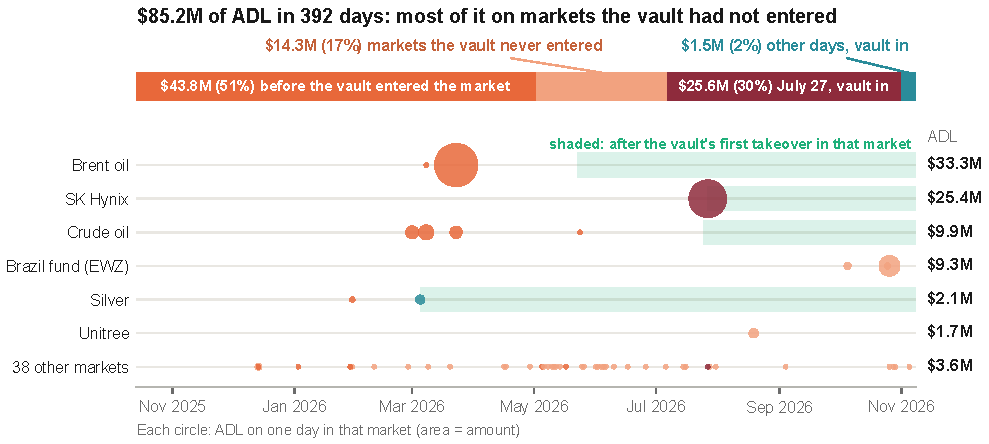
\includegraphics[width=\textwidth]{figs/adl_timeline.pdf}\end{center}
\vspace{-1.5ex}

Most of the rest is one day: SK Hynix on July 27 (\$25.6M, 30\% of the total; the chart's SK Hynix row, \$25.4M, leaves out \$160k on a second SK Hynix market). There the vault was allowed in but its balance was not enough: what we read as a wrong price at the reopening dragged the mark down, and in our replay the vault needed \$1.43M against a balance of about \$1.04M five days earlier (page~\pageref{sec:skhx2}). The remaining \$1.5M is silver on March 5, a day when the vault did take a position and ADL happened all the same.

\foot
\begin{exact}[The rule, as replayed]
On markets where the vault is allowed in (cross margin enabled), a position whose equity falls below two thirds of its maintenance margin leaves the order book: the vault takes it at the bankruptcy price, where its equity is zero. On isolated-only markets the order book keeps selling, and the position is auto-deleveraged against profitable traders only once its equity is negative, as trade.xyz's documentation describes; in our replay, at the previous update's mark, as on the chain. Counts: \S\ref{sec:cover}.
\end{exact}

%======================================================================================== 4 lagging mark
\page{In a crash, today's mark arrives about a minute late}{Problem 2: backstop loss}\phantomsection\label{sec:lag}

On October 28 Alphabet reported earnings after the close and its share price fell about 7\% within a minute. On xyz, the prices trade.xyz publishes may move only 0.5\% toward the external price at each update, about every three seconds, so for the next minute the mark stayed far above what the share was really worth.

While the mark is too high, positions that are already lost are not liquidated: on paper they still look solvent. When the mark finally catches up they can be far past the point where the order book could close them, and go straight to the vault.

\begin{center}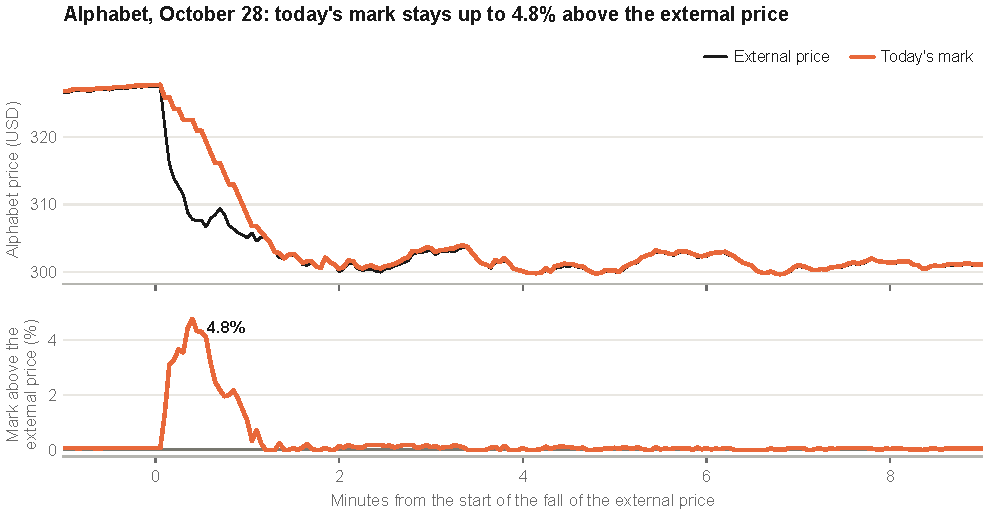
\includegraphics[width=\textwidth]{figs/crash_mark.pdf}\end{center}
\vspace{-1.5ex}

The lower panel shows the gap: today's mark stays up to 4.8\% above the external price for about a minute. On the three crashes replayed, 814 of 819 takeovers reach the vault already below the external price (worth less than zero at that price). Change 1 (page~\pageref{sec:vote}) brings the mark down with the external price; whether that lightens the vault's load differs from crash to crash (page~\pageref{sec:res-mark}).

\foot
\begin{exact}[Today's rule, as we reconstruct it from the chain record]
\emergencystretch=1.5em\hbadness=1500 The relayer publishes an \emph{oracle} price (its own copy of the external price, used for funding), $O_t = \D_t\big(\clip(E_t,\ O_{t-k}(1\pm c))\big)$ with $c = 0.5\%$ per update, and two mark inputs, the first the oracle clipped around the previous mark on the chain, the second the external price plus the book's premium; Hyperliquid takes the median of those two and xyz's book price. The documentation gives the median and the 0.5\% clamp; the read lag $k$, the clip around the previous mark and the bound on the inputs are what the chain shows (symbols: page~\pageref{sec:formulas}). Full rules: \S\ref{sec:current}.
\end{exact}

%======================================================================================== 5 change 1
\page{Change 1: the mark becomes the middle of three votes; in the tests a short wrong price barely moved it, a lasting one moves it slowly}{Serves problem 2 (backstop loss), in the replay of July 27 less money to avoid ADL (indeterminate, page~\pageref{sec:skhx2}), and the condition ``attacks do less harm'' \,·\, a change for trade.xyz}\phantomsection\label{sec:vote}

\changerule{$M_t = \clip\big(\med(X^1_t, X^2_t, B_t),\ M_{t-1}(1\pm 1\%)\big)$, where the oracle moves toward the external price $E$ by at most $0.5\%$ per update and the first input follows the mark}
{$M_t = \clip\big(\med(\nw{V_t},\ \nw{A_t},\ B_t),\ M_{t-1}(1\pm 1\%)\big)$: the feed's vote $\nw{V_t}$ (the external price itself) and the anchor $\nw{A_t}$ (its 30-minute average); Hyperliquid's formula is unchanged}

At every update the mark is the middle one of three votes. They are not independent: the anchor is tied to the feed and the last mark, and a feed that is not live votes with xyz's book. \textbf{In the three crashes replayed, the crash was followed within seconds:} the external price and xyz's book fell together and two votes agreed. The design assumes the book follows a real move; if not, the mark follows at the anchor's pace, slower than today. \textbf{In the tests a short wrong price was outvoted:} it moves one vote, the book stays, and the anchor follows only at its 30-minute pace, so a lasting one moves the mark slowly. One wrong price followed by no further change is not outvoted. After two unchanged updates the feed counts as not live, and the internal price starts from the wrong value (page~\pageref{sec:notlive}); overnight, when the feed rarely changes, this is the ordinary case. \textbf{A push of xyz's book} is outvoted while the feed and the anchor agree.

\begin{center}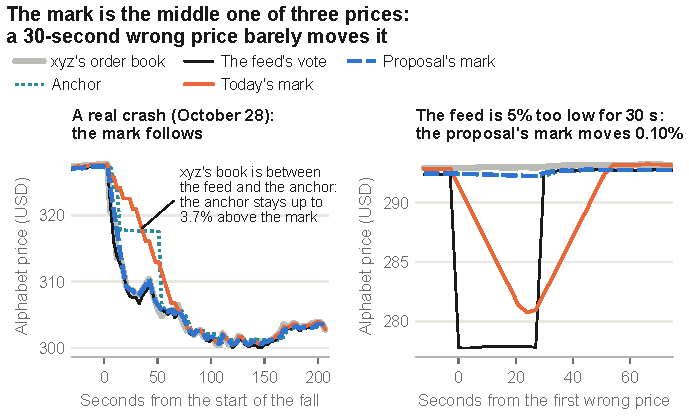
\includegraphics[width=.68\textwidth]{figs/mark_changes.pdf}\end{center}

\textbf{The correction step} pulls the anchor back between the feed's vote and the last mark, unless xyz's book lay between them; then it can lag (Alphabet crash: 13 updates, up to 3.66\% above the mark). Its cost: if xyz's book dips while a wrong price lasts, the mark keeps much of the dip (Alphabet, 20\% wrong price and a 45-second \$5M push: after two minutes 16.14\% today, 9.32\% with the step, 1.57\% without). Its use: a \$5M push held five minutes in a crash needs \$899k of capital today, \$840k with the step, \$1.188M without (\S\ref{sec:three}, page~\pageref{sec:three}).

\foot
\begin{exact}
Feed's vote: $V_t = E_t$ if the feed is live (the venue is open and $E$ changed in at least one of the last two updates), else $O_t$ (change 2); with the feed live $O_t = \D_t(E_t)$.
Anchor: $\tilde A_t = A_{t-1} + \big(1 - e^{-\Delta t/\tau}\big)(V_t - A_{t-1})$, $\tau = 30$\,min, $A_0 = E_0$; $A_t = \tilde A_t$ if xyz's book price $B_{t-1}$ was strictly between $V_{t-1}$ and $A_{t-1}$, else $A_t = \clip\big(\tilde A_t,\ [V_t, M_{t-1}]\big)$. The anchor is never restarted and is exempt from the discovery bound; it is one of the two published inputs. Inputs and open points: \S\ref{sec:three}, page~\pageref{sec:three}.
\end{exact}

%======================================================================================== 6 change 2
\page{Change 2: when the feed is not live, a short push moves the mark slowly; one held for hours still moves it}{Serves the condition ``attacks do less harm'' \,·\, a change for trade.xyz}\phantomsection\label{sec:notlive}

\changerule{in scheduled closures or after a data gap (15\,s for Korean stocks, 30\,s for FX): $O_t = O_{t-1} + \big(1 - e^{-\Delta t^*/\tau}\big)(\text{mid}_t - O_{t-1})$, the book's mid standing in for the documented impact price (the fill price of a set order size)}
{in closures \nw{or when $E$ has not changed for two updates}: $O_t = O_{t-1} + \big(1 - e^{-\Delta t^*/\tau}\big)\,\nw{\clip\big(\text{mid}_t - O_{t-1},\ \pm\kappa\,O_{t-1}\big)}$, $\kappa = 1\%$, $\tau = 30$\,min}

When the asset's own market is closed (weekends, the futures' daily break, the Korean night), xyz prices the market from its own book. Today that internal price is already a 30-minute average of the book with no cap, but the mark's two other inputs follow the book at once, so a push of a few minutes drags the mark and liquidates other traders.

The change: one rule whenever the feed is not live, closure or repeated value. The internal price's pull toward the book is capped (about 2\% per hour), and it becomes the feed's vote of change 1, so no input follows the book at once. Overnight this is the normal regime; in regular hours it is on for 3 to 5 seconds at a time (\S\ref{sec:three}, page~\pageref{sec:three}).

\begin{center}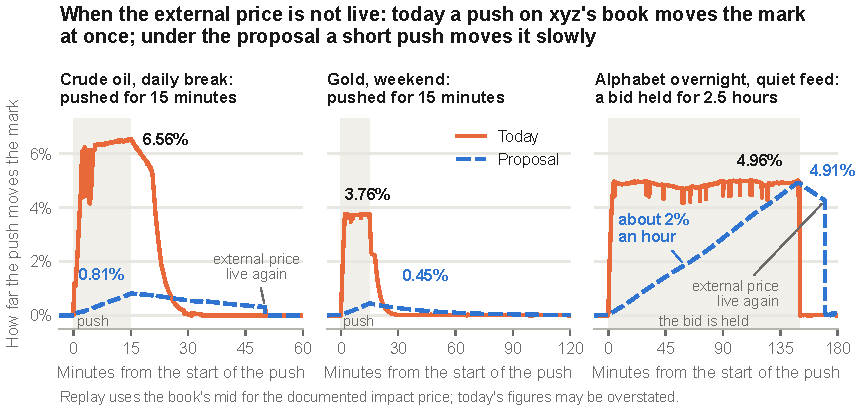
\includegraphics[width=.87\textwidth]{figs/closed_attacks.pdf}\end{center}
\vspace{-1.5ex}

Each push is measured from the path without it (crude oil: $-0.32\%$ without, $+0.48\%$ with, a gap of 0.81\% as measured). After the push the proposal's mark returns more slowly than today's. \textbf{Only with change 1:} alone under today's mark the cap leaves a push as effective as today (6.56\%, 6.48\%), since the mark's other inputs still follow the book. \textbf{What it does not stop:} a push kept up for hours moves the mark as far as today's does in five minutes. trade.xyz re-anchors the discovery bound near its edge (``resets''); our replay has none under either rule set, nor does change 2 as written; they could be kept.

\foot
\begin{exact}
Whenever the market is in a scheduled closure, or $E_t = E_{t-1} = E_{t-2}$: $O_t = O_{t-1} + \big(1 - e^{-\Delta t^*/\tau}\big)\,\clip\big(\text{mid}_t - O_{t-1},\ \pm\kappa\,O_{t-1}\big)$, $\kappa = 1\%$, $\tau = 30$\,min, with the mark formula of change 1. When the feed stops being live, the internal price starts from the last external price, even one that has just printed (as at 23:00 on July 27), and stays within $E_{\text{last}}(1\pm d)$. If the external price changes inside a scheduled closure, the bound moves but the internal price does not restart (as at 17:17 on July 27). $\kappa = 1\%$ is Hyperliquid's own per-update limit, as close at reopening as today on 510 closures (\S\ref{sec:closed}).
\end{exact}

%======================================================================================== 7 change 3
\page{Change 3: cut a large position back to its initial margin at once; it helps only with change 1, and the vault still inherits more than today}{Serves problem 2 (backstop loss) \,·\, needs a Hyperliquid change}\phantomsection\label{sec:cutback}

\changerule{below maintenance margin and above \$100k: a first order for $20\%$ of $|q|$, then full-size orders during a 30\,s cooldown}
{below maintenance margin and above \$100k, at \nw{every update}: sell $\nw{\Delta q = \big(1 - \text{equity}/\text{IM}\big)\,|q|}$, enough to restore the initial margin IM at the market's maximum leverage}

Hyperliquid's documentation says a position above \$100k that falls below its maintenance margin first has 20\% sold. If it is still below within the next 30 seconds, the rest is sold in full. As we reconstruct it, after 30 seconds a new round starts with 20\% again. (trade.xyz's page describes only full-size orders.) However far the price has moved, the first sale is small; if the position keeps losing, what is left is then closed in one block, often into a thin book.

The change: at every mark update, sell exactly what brings the position back to the initial margin at the market's maximum leverage. When a position first crosses its margin requirement today's rule sells a fifth of it, this one about half: more is sold early, while the book can still take it, and less is left for when the price falls.

\begin{center}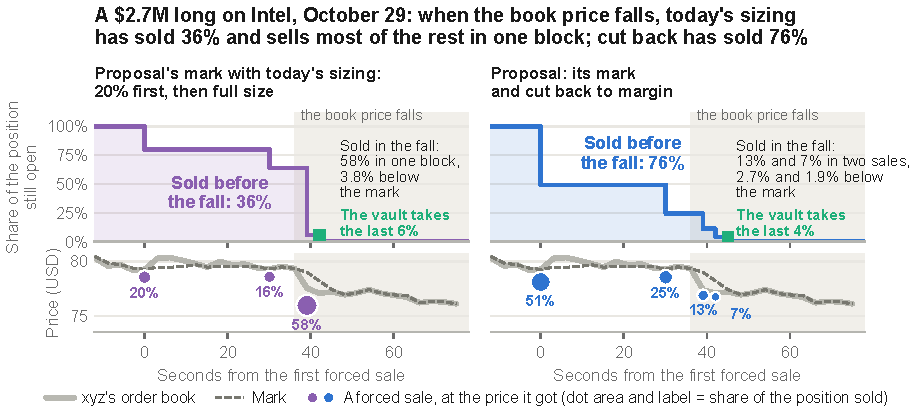
\includegraphics[width=.92\textwidth]{figs/cutback_how.pdf}\end{center}
\vspace{-1.5ex}

Both are replayed here with the proposal's mark. xyz's book price holds for about half a minute and then falls. By then today's sizing has sold 36\% of the position and the cut-back 76\%; today's sizing then sells 58\% in one block, 3.8\% below the mark. Part of that fall is the liquidations themselves. This is the clearest of the 23 large positions, not a typical one.

\textbf{Why only after change 1.} With today's mark, which lags a crash, the cut-back is sized from a position value that is too optimistic, and it leaves the vault more, not less. Even with change 1, on the 23 largest positions the vault inherits more than today (\$8.72M today, \$9.78M; change 1 alone, \$11.76M), while isolated-only ADL falls (\$300.4k, \$99.5k). What the tests showed, and what the cut-back costs: page~\pageref{sec:res-cut}.

\foot
\begin{exact}
$q_{\text{sold}} = \min\{q : \text{equity} \ge \text{IM}(q_{\text{left}})\}$ at each mark update, for positions above \$100k, with no cooldown; in closed form $\Delta q = (1 - \text{equity}/\text{IM})\,|q|$. Other targets (maintenance margin, 1.5 and 3 times it, all sizes) left the vault more, or forced more liquidation; details in the companion note.
\end{exact}

%======================================================================================== 8 change 4
\page{Change 4: a candidate list of six markets that clear the bar of those the vault already serves}{Serves problem 1 (ADL) \,·\, a trade.xyz setting, reviewed by Hyperliquid's validators}\phantomsection\label{sec:five}

\changerule{the vault may take positions in 22 markets; the other 98 are isolated-only, with ADL as their only backstop}
{the vault may also take positions in \nw{Robinhood, MicroStrategy, Nebius, AMD, the Korea fund EWY and Samsung} (28 markets)}

Hyperliquid's HIP-3 documentation says validators accept the vault only on assets with enough liquidity, a reliable external price and resistance to manipulation; the switch is irreversible. It adds to what the vault may carry, within each market's open-interest cap, and traders would notice one thing: cross margin becomes the default, and a backstop takeover of a cross account moves all its cross positions to the vault.

It gives two thresholds: a 50\% move in a day triggers a review of trade.xyz's stake, and 50\% daily moves more than once a month make a market ineligible. For the rest we take the weakest of the 22 markets the vault serves today: a listed underlying, at least Amazon's trading volume on xyz (median \$8.0M a day over the 209 days for which we have hourly prices), no 50\% day, and no day larger than SanDisk's largest (35\%; detail: \S\ref{sec:cover}). Six of the 98 isolated-only markets pass: Robinhood, MicroStrategy, Nebius, AMD, the Korea fund EWY and Samsung, together a quarter of the open positions on isolated-only markets. EWY and Samsung are Korean, like SK Hynix.

\begin{center}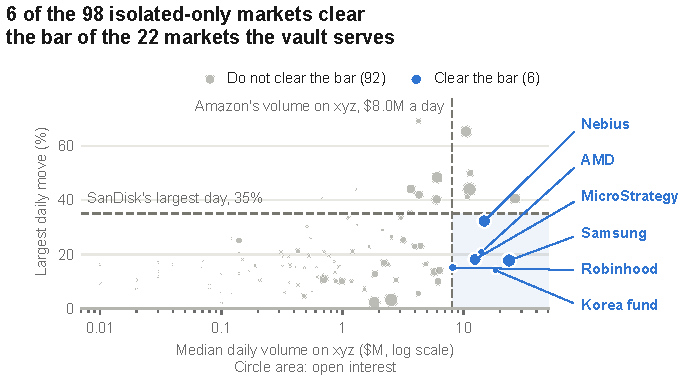
\includegraphics[width=.7\textwidth]{figs/eligibility.pdf}\end{center}
\vspace{-1.5ex}
\vspace{1ex}
\textbf{What the chart shows.} Each circle is one market (area: open interest); the six that clear every bar are the ones change 4 names.

\par{\small\color{mute}Sources: market list read from Hyperliquid on November 2, 2026; volume and daily moves over 209 days; detail: \S\ref{sec:cover}.\par}
%======================================================================================== 8b ceiling
\page{Change 4's case is forward-looking: the six markets cut an upper bound of ADL by up to 45\%; in the one replay, \$64k to \$60k}{Serves problem 1 (ADL) \,·\, what change 4 would and would not have done}\phantomsection\label{sec:ceiling}

The chart applies each of xyz's five worst real 1-hour and 4-hour moves to today's open positions as one instant move. For each it shows the ADL on isolated-only markets today, and with the vault allowed in the six markets. The reduction runs from none to 45\% (\$4.11M to \$2.25M, July 29), depending on the window. It assumes the vault can absorb what it would inherit; its capital for the six was not computed (the only indication: with cross margin on every isolated-only market, the 4-hour worst case rises from \$3.0M to \$5.6M, \S\ref{sec:cover}).

\begin{center}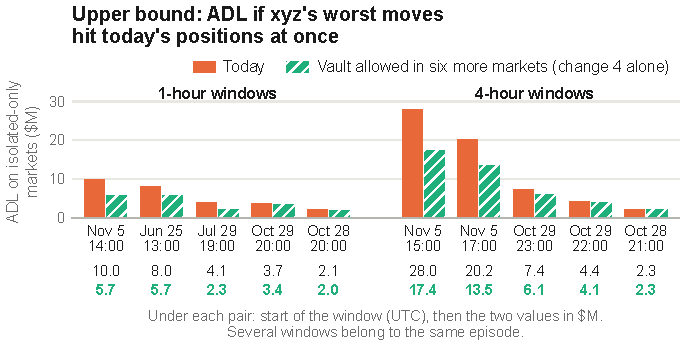
\includegraphics[width=.7\textwidth]{figs/six_markets.pdf}\end{center}
\vspace{-1.5ex}

\textbf{The chart is a ceiling, not an estimate:} in a real hour the book liquidates most positions before ADL is reached. On November 5, the one such day we replayed, ADL on isolated-only markets was \$154k under today's rules (\$154k on the chain), against \$10.0M to \$28.0M in that day's bars; under the proposal it was \$64k, and \$60k with the vault also in the six markets.

\textbf{This change would not have prevented the ADL on record:} the six had \$20.7k of the \$85.2M. Most fell on markets the vault serves today, and most of the rest on EWZ (page~\pageref{sec:adl}), which does not clear the bar.

\par{\small\color{mute}Sources: open positions and price history of xyz; the November 5 replay of 33 markets: page~\pageref{sec:users}; detail: \S\ref{sec:cover}.\par}

%======================================================================================== 9 change 5
\page{Change 5: a capital floor; today's ten-year level, \$1.85M, is about what the vault holds and would not have covered July 27}{Serves problem 3 (too little capital) \,·\, a suggestion to trade.xyz, not a protocol rule}\phantomsection\label{sec:capital}

\changerule{no published rule ties the vault's size to the positions it backs; it holds \$1.84M}
{a \nw{floor to discuss}: at least the once-in-ten-years value of \nw{$C(\mathcal{P}, r)$}, the capital to carry what the vault would take after a move $r$ of all markets, \nw{recomputed every morning}; more is trade.xyz's choice}

How much the vault holds is trade.xyz's decision, so we offer only a lower bound. We found no published rule. The suggestion: each morning, move the markets, see which positions the vault would have to take, and add up the margin it would need to carry them.

\textbf{The method.} The left panel moves every market by the same amount at once. The right panel applies each of about 5{,}000 real hours of xyz's 120 markets (209 days) to today's positions, all markets together; each day keeps its worst hour. A standard extreme-value curve (a generalized Pareto, the method behind ``100-year flood'' estimates: \href{https://doi.org/10.1111/j.2517-6161.1990.tb01796.x}{\textcolor{prop}{Davison and Smith, 1990}}; \href{https://doi.org/10.1007/978-1-4471-3675-0}{\textcolor{prop}{Coles, 2001}}) is fitted to the largest 15\% of those 209 daily figures, about 31 points, and read at the level exceeded once in ten years; the whiskers are the 90\% range over 500 refits on resampled days. This is an estimate, not a tested result: with 31 points no significance test can support a ten-year level. A backtest fitted on the first 125 days predicted 0.8 days above \$500k in the next 84; there were 3, a gap with about a 5\% chance if the curve were right. In the tail it errs low.

\begin{center}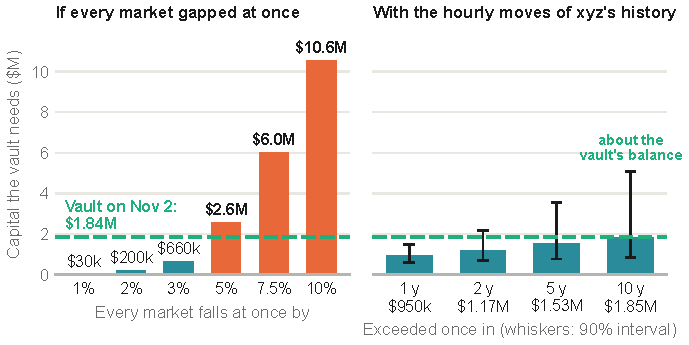
\includegraphics[width=.68\textwidth]{figs/capital.pdf}\end{center}
\vspace{-1.5ex}

\textbf{What it gives today, as an illustration.} The once-in-ten-years need is \$1.85M (range \$830k to \$5.1M), close to the \$1.84M the vault holds. The ten-year floor would not have covered July 27. That day the vault needed \$2.60M to carry what it inherited under today's rules (\$1.43M only to avoid ADL, page~\pageref{sec:skhx2}). The model moves prices in one instant, so it leaves out crashes driven by the path of the mark; and it is fitted to each day's worst hour, so xyz's worst real 4-hour move, which on today's positions needs \$3.0M, lies beyond it. What we suggest is the method, as a floor to discuss with its range, not these figures: the floor firms up as the history grows, and trade.xyz may hold a longer history.

\foot
\begin{exact}
$C(\mathcal{P}, r) = \sum_{\text{taken}} \frac{|q|\,P'}{2\,\text{maxLev}} - \sum_{\text{taken}} \text{eq}'$, with $P' = P(1+r_m)$ ($r_m$: the move of market $m$) and a position taken when $\text{eq}' < \tfrac23\,\text{MM}'$: the capital for the vault to stay above its own maintenance margin after an instant move $r$ of all markets. Positions: 100{,}512, as of October 30, 2026; the vault's \$1.84M, November 2. Backtest, worst cases and limits: \S\ref{sec:cover}.
\end{exact}

%======================================================================================== 10 change 6
\page{Change 6: the external price is often unchanged overnight; three items would make it easier to check}{Serves the condition ``attacks do less harm'' \,·\, trade.xyz's price pipeline}\phantomsection\label{sec:feed}

\changerule{one published external price $E$, with no age; for US stocks trade.xyz's documentation names one venue for the overnight session, Blue Ocean ATS (an alternative trading system for US stocks at night), and does not say how the price is computed}
{$E$ \nw{published with its age} and \nw{what it is built from in each session}; overnight, \nw{a minimum size} for what moves it; \nw{a move checked} against trade.xyz's other sources before it is published, if this is not already done}

How much of the defense against a wrong external price lies in the feed itself? With change 1 a manipulated external price moves the mark by itself only slowly (after 15 minutes of a 20\% error: 16\% at once today, 7.92\%). It is still one vote of three, and an attacker who walks it needs only one more, xyz's book, cheap to push on every market we measured (page~\pageref{sec:attacks}). We think the main defense lies in how the external price is built.

What the record shows is that the external price is often unchanged from one update to the next. Overnight, a session for which trade.xyz's documentation names one venue (Blue Ocean ATS), the published price is unchanged on most updates: on half of the market-nights it is unchanged on more than 78\% of updates (74.9\% of all overnight updates taken together). In regular hours the same figure is 30\%. An unchanged price may simply mean no new trade or quote: for US stocks how the price is computed and filtered is not documented, so we judge it only by what the chain record shows. For indices, commodities, FX and non-US stocks the documentation does give the derivation, so item 1 below (stating what the price is built from) is partly in place there.

\begin{center}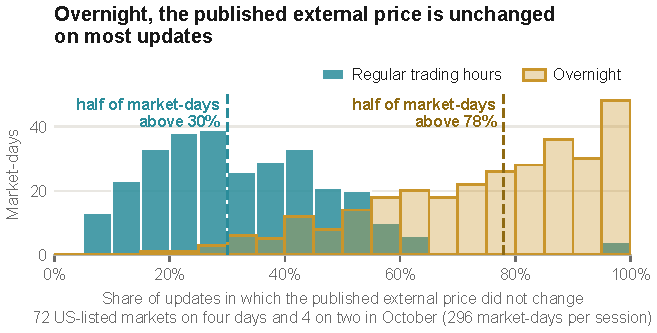
\includegraphics[width=.66\textwidth]{figs/feed_age.pdf}\end{center}
\vspace{-1.5ex}

\textbf{Three items,} some perhaps already in place.
\begin{enumerate}[leftmargin=1.5em,itemsep=.3ex,topsep=.3ex]
\item \textbf{Publishing the age of the price} with every update (a field or a document), and stating what it is built from in each session. Change 2 treats an unchanged price as not live; an explicit age would make that exact.
\item \textbf{Requiring a minimum size for what moves the overnight price,} if that is not already the case. For US stocks we do not know how the price is computed, so we cannot tell whether a small trade can move it today.
\item \textbf{Checking a move against the other sources trade.xyz draws on before publishing it,} if this is not already done, and holding a move that nothing else confirms.
\end{enumerate}

\par{\small\color{mute}Sources: 76 US-listed names, October 20, 21, 28 and 29: 296 market-days per session (72 markets on four days, 4 on two); walks: page~\pageref{sec:attacks}.\par}

%======================================================================================== 11 steps
\page{The changes could ship in steps: 1 and 2 together, the cut-back after them, 4 with the capital it needs, 5 and 6 at any time}{How the suggestions fit together}\phantomsection\label{sec:steps}

The six changes are not a single package to accept or refuse whole. They can be taken in steps, or in part.

{\normalsize\renewcommand{\arraystretch}{1.25}
\begin{tabularx}{\textwidth}{@{}r>{\raggedright\arraybackslash}p{4.6cm}>{\raggedright\arraybackslash}p{2.4cm}>{\raggedright\arraybackslash}X@{}}
\toprule
 & Change & On its own? & Why\\
\midrule
1 & Mark is the middle of three votes & With 2 & Change 1 was never replayed with today's internal price\\
2 & One rule when the price is not live & Only with 1 & Alone, under today's mark, a push lifts the mark as much as today (6.56\% today, 6.48\%); with change 1 it supplies the feed's vote\\
3 & Cut-back, not today's sizing & After 1 & With today's mark it leaves the vault more\\
4 & A candidate list of six markets for the vault & Yes, with capital & A market setting, but the vault's capital for the six was not computed (change 5)\\
5 & A floor for the vault's capital & Yes & A suggestion to trade.xyz, not a protocol rule\\
6 & External price: age, sources, minimum size, cross-check & Yes & A change to the price feed\\
\bottomrule
\end{tabularx}}


\vspace{1.5ex}
\textbf{What each one is for.} Changes 1 and 2 make the mark follow a real crash and keep a wrong price to one vote. Change 3 sells a large position in trouble sooner, in larger pieces, once the mark follows the crash. Change 4 would put the vault before ADL on six markets that clear the bar of those it already serves. Change 5 suggests a floor for the vault's capital. Change 6 looks after the external price, the one vote that comes from outside xyz.

Where the suggestions do not help, or do worse than today: page~\pageref{sec:costs}.

\foot
\begin{exact}[Where the rules are]
Each change's rule is in the Today / Suggested lines of its page. Today's rules and the suggested ones side by side: page~\pageref{sec:formulas}; in full: \S\ref{sec:current} and \S\ref{sec:three}, page~\pageref{sec:three}; earlier variants: the companion note on earlier variants. Changes 5 and 6 are not trading rules. Change 1 with today's internal price was not replayed; change 2 alone under today's mark was replayed, and does not protect the mark (page~\pageref{sec:notlive}).
\end{exact}

%======================================================================================== 12 method
\page{What was tested: a replay whose mark matches the chain's at 98\% or more of liquidation blocks on the days checked; hard days and thirty random ones}{What was tested \,·\, what the comparisons rest on}\phantomsection\label{sec:tests}

\textbf{A replay engine, built from outside.} trade.xyz's relayer is not public, so today's rules are our reconstruction from the chain record and trade.xyz's documentation. We rebuilt Hyperliquid's clearing rules in code; a proposed rule is a switch in that engine, so two results differ only by the rule. Under today's rules it gives the same mark as the real chain at 98 to 100\% of the blocks where a liquidation occurred, on seven market-days (the mark, not every outcome: see November 5, page~\pageref{sec:users}), 966 of 974 in all (99\%), and at 162 of 165 (98\%) on the five isolated-only ADL days, and reproduces 41 of the 42 real vault takeovers on crude oil (one missed, two added, the same \$500k). (Page~\pageref{sec:res-mark} counts takeover events: crude oil's 49 today come from 43 accounts.) Where we have a rule wrong, trade.xyz will see it first.

\textbf{The data, all public.} Hyperliquid's node archive gives each day's full command stream, including every update trade.xyz's relayer sent. Hydromancer, a third-party data service, keeps an archive of xyz with real fills, position snapshots and the book by the minute; its 392 days give the ADL and takeover counts. A replay applies every recorded command in order from a snapshot; the book does not react to our mark.

\textbf{Why we expect the result beyond these days.} A handful of examples is usual for such a study; the reason to expect more is a mechanism. Today's mark lags a fast move by construction (0.5\% per update against several percent in a minute), so positions already lost are not liquidated until it catches up and reach the vault further below water; a mark that follows the move reaches them earlier, whatever the market or the day. The size of the gain depends on the move's speed and the book's depth, so it differs by crash (large on Intel, reversed on Alphabet). This is an expectation, not a finding: days chosen after the formula was fixed, and the large ADL days we did not replay (Brent, crude oil, EWZ), would test it.

\textbf{Real days: most chosen to hurt, thirty drawn at random.}

{\small
\begin{tabularx}{\textwidth}{@{}>{\raggedright\arraybackslash}X>{\raggedright\arraybackslash}p{6.4cm}@{}}
\toprule
Days replayed & What they test\\
\midrule
Alphabet October 28; Intel, Amazon October 29 (3) & Earnings crashes: the mark in a fast fall\\
SK Hynix July 27 (1) & The largest real ADL: a wrong price at a reopening\\
Oil, gold, silver, Alphabet, Meta, SpaceX on September 10, October 22 and October 30 (7) & Held out at first; the oil days later shaped change 2\\
Alphabet, Intel, Amazon on October 20 and 21 (6) & Quiet days\\
The rest of the three crash days, outside regular hours and the crash window (60\,s before the fall to 30\,min after) & Traders should see little difference\\
ServiceNow, Lumentum, Marvell October 28; Reddit October 29; Cloudflare November 5 (5) & ADL on isolated-only markets\\
The same days with a wrong price, a walked price or a pushed book; crude oil's daily break; gold's weekend & Attacks\\
33 markets together on November 5 & A whole day, 33 markets at once\\
30 market-days drawn from July 1 to November 8 (used: August 4 to October 1) & Days we did not choose\\
The full record of xyz fills, 392 days & Where every backstop event really went\\
\bottomrule
\end{tabularx}}

\vspace{1ex}
\textbf{Results that we can rebuild.} The 22 market-days counted in the table were rebuilt on November 11 and every test run again on them: the \emph{final run}, on which every figure here rests. Parity by day: page~\pageref{sec:appintro}; specification and test vector: \S\ref{sec:three}.



%======================================================================================== 13 results mark
\page{Test results: in the three crashes the vault gets positions earlier; money to avoid ADL falls in total and on Intel, and rises on Alphabet}{What was tested \,·\, changes 1 to 3}\phantomsection\label{sec:res-mark}

What does the proposal change for the vault? By the ranking of page~2, what matters is the money to avoid ADL and the capital, more than the amount inherited. We replayed the three earnings crashes and the other tests under both rule sets; each line is one test. \emph{Money to avoid ADL}: what the vault must hold so that its account never falls below zero, where traders are auto-deleveraged. \emph{Capital the vault needs}: what it must hold to keep its own maintenance margin on what it carries; it can be large when the first is small. ADL is triggered when the vault's account value would go below zero, so the first is the one that decides it. Lower is better; more inherited can mean positions taken earlier.

{\renewcommand{\arraystretch}{1.2}
{\small
\begin{tabularx}{\textwidth}{@{}>{\raggedright\arraybackslash}Xrrrr@{}}
\toprule
Three crashes, today $\rightarrow$ proposal & Capital the vault needs & Money to avoid ADL & Inherited by the vault & Takeovers below $E$\\
\midrule
Alphabet, Oct 28 & \$329k $\rightarrow$ \$419k & \$185k $\rightarrow$ \$219k & \$6.96M $\rightarrow$ \$10.28M & 156/158 $\rightarrow$ 12/258\\
Intel, Oct 29 & \$244k $\rightarrow$ \$45k & \$166k $\rightarrow$ \$33k & \$2.24M $\rightarrow$ \$300k & 258/258 $\rightarrow$ 23/29\\
Amazon, Oct 29 & \$143k $\rightarrow$ \$125k & \$112k $\rightarrow$ \$99k & \$1.55M $\rightarrow$ \$1.32M & 400/403 $\rightarrow$ 287/296\\
Total & \$715k $\rightarrow$ \$589k & \$462k $\rightarrow$ \$352k & \$10.75M $\rightarrow$ \$11.90M & 814/819 $\rightarrow$ 322/583\\
\bottomrule
\end{tabularx}}

\textbf{What the vault is handed.} Most takeovers reach the vault below the external price today (table, and page~\pageref{sec:lag}); under the proposal about half do. Valued at the external price when handed over: $-\$157.9$k today, $+\$63.4$k under the proposal. This is the state of positions on arrival, not the vault's result; the sums are of the order of the replay's own error, so the counts carry the weight. The change comes from the mark, not the way of selling; Amazon stays mostly below under both. On Alphabet the vault inherits more and needs 27\% more capital and 18\% more money to avoid ADL; we think because it gets positions earlier, while they still have value. The gain in the total comes from Intel.

{\small
\begin{tabularx}{\textwidth}{@{}>{\raggedright\arraybackslash}Xrr@{}}
\toprule
Other tests, replayed under both sets of rules & Today & Proposal\\
\midrule
SK Hynix, July 27: money to avoid ADL (page~\pageref{sec:skhx2}) & \$1.43M & \$892k\\
Five replays of isolated-only markets (mark as on the chain at 162 of 165 liquidation blocks): ADL & \$300.4k & \$99.5k\\
Held out at first: takeovers on two oil markets, September 10 (later shaped change 2; 89 and 6 accounts counted market by market, 88 and 6 distinct wallets) & 95 & 13\\
\quad on the five other market-days (4 and 7 accounts, by either count) & 8 & 11\\
\quad positions the vault inherits, oil / five others & \$1.25M / \$5k & \$84k / \$100k\\
\bottomrule
\end{tabularx}}




\vspace{1ex}
}


\par{\small\color{mute}Accounts counted market by market count a trader once in each market; distinct wallets count each trader once across all markets. Sources: every test, with the wrong prices, walks and pushes of page~\pageref{sec:attacks}: \S\ref{sec:three}, page~\pageref{sec:three}; closures: \S\ref{sec:closed}.\par}

%======================================================================================== July 27
\page{Test results: on July 27 the proposal's mark followed xyz's book, not the wrong prices; in the afternoon it sat up to 7\% above the book}{What was tested \,·\, SK Hynix, the largest ADL on record (\$25.6M)}\phantomsection\label{sec:skhx}

SK Hynix on July 27 is the largest ADL on record. We replayed the whole day under both rule sets to see what the proposal's mark would have done. \textbf{The afternoon.} The external price stood at 1,237.30 from 11:00 until 17:17:45\,UTC, then printed 1,113.60 ($-10\%$) during the Korean night, 1,237.30 $\times$ 0.90 rounded to the price grid: we read it as trade.xyz's 10\% bound being re-anchored, not a market price. xyz's book had already fallen to 1,117. Today's mark stayed within 0.93\% of the book. The proposal's internal price moves at most about 2\% an hour, so its mark lagged the falling book: between 11:00 and 23:00 it was more than 2\% above the book on 20.9\% of updates (about 2.5 hours), more than 5\% above on 3.2\%, and at most 7.03\% above. That is a cost of change 2: longs were marked above what they could sell at, and today's rules liquidated 156 different accounts through the book where the proposal liquidated 121, counted once across both afternoon phases (35 fewer, \$262k less). trade.xyz's changelog says shortening its internal time constant reduces the gap between traded price and oracle; change 2 goes the other way.

\textbf{The reopening.} At 23:00:03 the external price printed 868.18, 22\% below its last value, for two minutes. xyz's book, as recorded, fell from 1,128 to 955 in 24 seconds (its low was 951). \textbf{That 955 sat at the edge of today's bound:} today's published inputs were 954.99 on one update and 954.98 on the next two, the edge of a 10\% bound around the wrong price (868.18 $\times$ 1.10), before falling; from 23:00:27 the book's best bid sat at 954.98, and from 23:00:33 its best ask at 954.99. Under today's rules the mark falls 1\% per update to 917 by 23:01:18. Under the proposal the wrong price is outvoted, the anchor falls from 1,131 to 1,114 in the two minutes, and the median is the book: the mark follows it to 955 at 23:01:03, and no further. At 23:02:03 the external price printed 1,198.50; three seconds later the book was back near 1,107; today's mark rose to 1,197, the proposal's stayed at 1,128 or below to 23:08.

\begin{center}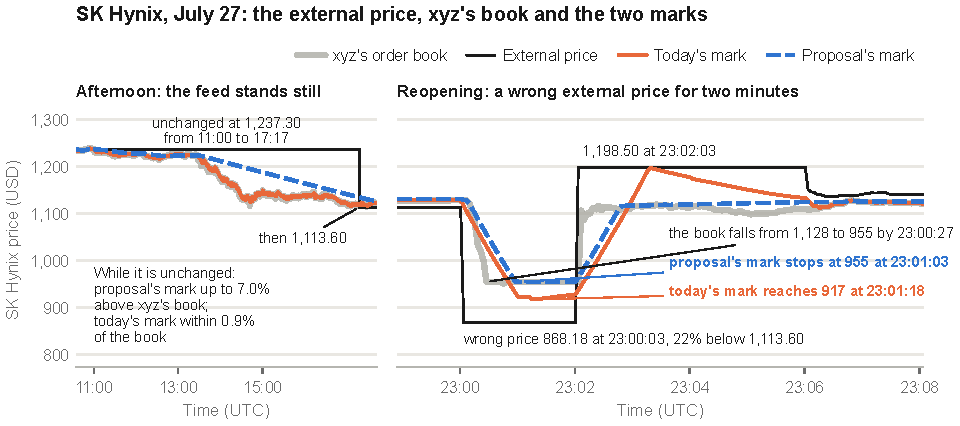
\includegraphics[width=.94\textwidth]{figs/skhx_0727.pdf}\end{center}
\vspace{-2ex}

\textbf{What this shows.} The mark did not follow either wrong price, but the book fell 15\% and the mark went with it, bottoming 4\% higher than today's (917 today, 955). The outcome is indeterminate: had the book followed the proposal's published 868, the proposal's mark could have gone below today's 917. Costs and savings: next page.

\par{\small\color{mute}Sources: the final run, with the proposal as written; the day's inputs and outputs are a test vector with the code.\par}

%======================================================================================== July 27, costs
\page{Test results: July 27 is indeterminate: 38\% less money to avoid ADL on the recorded book, which today's rule held at 955}{What was tested \,·\, SK Hynix, July 27, phase by phase}\phantomsection\label{sec:skhx2}

The table splits the replayed day into its phases: what each set of rules liquidated through the book, handed to the vault, and needed to avoid ADL.

{\small\renewcommand{\arraystretch}{1.15}
\begin{tabularx}{\textwidth}{@{}>{\raggedright\arraybackslash}Xrr@{}}
\toprule
July 27, by phase & Today & Proposal\\
\midrule
11:00 to 17:17, book falling: liquidated through the book (accounts) / taken over & \$1.424M (156) / 0 & \$1.096M (101) / 4, \$10k\\
17:17 to 23:00: liquidated through the book / taken over & \$0 / 0 & \$66k (23) / 1\\
23:00 to 23:10, reopening: through the book / taken over & \$28.04M (901) / 351, \$15.90M & \$17.38M (765) / 586, \$18.97M\\
After 23:10: taken over & 1 & 4\\
Whole day: money to avoid ADL & \$1.43M & \$892k (38\% less)\\
Whole day: capital the vault needs & \$2.60M & \$2.27M (13\% less)\\
Takeovers below the external price at takeover (the external price was then the wrong one) & 349 of 352 & 586 of 595\\
\bottomrule
\end{tabularx}}

trade.xyz has since removed the Korean pre-market from external coverage (its changelog), so these pages show what the suggested rule would have done that day, not an open gap. \textbf{Less liquidated, more to the vault.} Over the day 17\% less is liquidated under the proposal (\$45.4M today, \$37.7M), but more of it reaches the vault and less goes through the book, and the extra takeovers come at the reopening, not in the afternoon. The afternoon lag left fewer accounts liquidated before the reopening (previous page; the table's 101 and 23 are 121 different accounts, since three are liquidated in both phases).

\textbf{ADL.} Money to avoid ADL falls 38\% and the capital the vault needs 13\% (page~\pageref{sec:res-mark} defines both). In the replay a balance like the \$1.04M the vault held five days earlier does not cover today's \$1.43M (and ADL did happen), but would have covered the proposal's \$892k. We do not claim ADL would have been avoided, only that this replay does not reach it. The margin is thin: \$892k needed against a balance of about \$1.04M five days earlier. The 38\% rests on a recorded book that today's rule held at 955 (page~\pageref{sec:skhx}). And the vault would have been far below its own maintenance margin, which needed \$2.27M. The difference comes from the mark, not the cut-back: with today's mark and the cut-back, money to avoid ADL is \$1.356M; with the proposal's mark and today's sizing, \$883k.

\textbf{The hold, left out.} Several earlier candidates need \$0 on this day because of a second rule, the \emph{hold}, which freezes the price band while the feed and xyz's book disagree. We left it out: it has three constants of its own, depends on reading xyz's trades and depth, and in earlier runs it could be frozen by an attacker's own wash trades (trading with itself at a chosen price) (\$50M lifted the mark 4.44\% in its first version). Its price is this page: \$892k where the hold gave \$0.

\par{\small\color{mute}Sources: the final run; whole-day figures and the two single-change runs (\$1.356M, \$883k): \S\ref{sec:three}, page~\pageref{sec:three}.\par}

%======================================================================================== 14 results cut-back and combinations
\page{Test results: the cut-back helps only with the proposal's mark and still leaves the vault more than today; the mark does most of the work on ADL}{What was tested \,·\, changes 1 to 3}\phantomsection\label{sec:res-cut}

What does the cut-back (change 3) add? We replayed each change alone and together on the 23 largest positions of the crashes and five isolated-only markets; change 1 always with change 2.

{\small
\begin{tabularx}{\textwidth}{@{}>{\raggedright\arraybackslash}X>{\raggedleft\arraybackslash}p{3.7cm}>{\raggedleft\arraybackslash}p{3.7cm}@{}}
\toprule
Rules switched on & Inherited by the vault (the 23 largest positions only) & ADL (five replays of isolated-only markets)\\
\midrule
None (today) & \$8.72M & \$300.4k\\
Cut-back only (3) & \$9.32M & \$301.1k\\
Proposal's mark with change 2 (1, 2) & \$11.76M & \$135.3k\\
Proposal's mark, change 2 and cut-back (1 to 3): the proposal & \$9.78M & \$99.5k\\
\bottomrule
\end{tabularx}}


\vspace{1ex}
The first column shows why change 3 waits for change 1: alone, under today's mark, the cut-back leaves the vault more than today; under the proposal's mark it leaves the vault less than the proposal's mark alone, but still more than today. The second column shows that the proposal's mark does most of the work on ADL and the cut-back adds to it. Why the vault receives more under the proposal's mark: page~\pageref{sec:res-mark}.

\begin{center}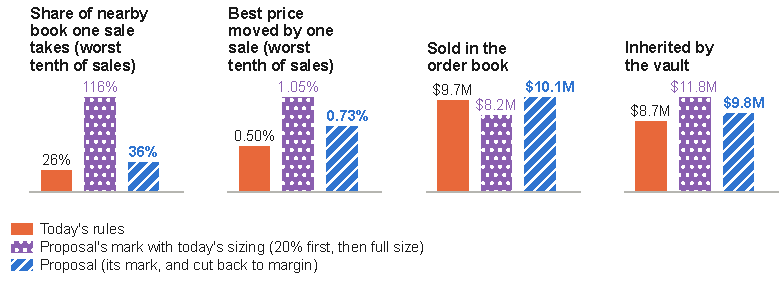
\includegraphics[width=.8\textwidth]{figs/cutback.pdf}\end{center}
\vspace{-2ex}
{\small\color{mute}The chart shows three configurations on the 23 largest liquidated positions of the three earnings crashes: today's rules, the proposal's mark with today's sizing, and the proposal.\par}

\textbf{What it costs.} Sales are larger (median \$47k today, \$53k with the proposal's mark and today's sizing, \$77k under the proposal; the first sale a fifth of a position, against about half), and filled further below the external price than today: on average 0.62\% today, 1.29\% under the proposal (1.44\% with the proposal's mark and today's sizing), because they sell into the fall. Compared with today's rules as a whole, the proposal's sales weigh more on the book: the worst tenth take 26\% of the nearby book today and 36\% under the proposal, and move the best price 0.50\% today and 0.73\%, because a mark that follows the crash liquidates into the fall and not after it.

\foot
\begin{exact}[Sources]
Inherited by the vault: the 23 largest liquidated positions of the three earnings crashes only, 21 of them the same under both marks. Sold plus inherited is \$18.4M today and \$19.8M under the proposal (\$19.9M with the proposal's mark and today's sizing), because each position is valued at the mark of its first forced sale, which comes earlier and higher: the positions' value at that first sale is \$18.9M today, \$20.4M under the proposal's mark. The extra inheritance is not valuation: at today's takeover prices the proposal's inherited positions are worth \$9.81M against \$8.72M (Alphabet: 21{,}653 shares today, 31{,}053). ``Nearby order book'': depth within 1\% of the best price. Under today's mark, fills are 0.62\% below the external price with today's sizing and 0.82\% with the cut-back. The four combinations: \S\ref{sec:three}, page~\pageref{sec:three}.
\end{exact}

%======================================================================================== 15 users
\page{Test results: on 30 random market-days about as many accounts are liquidated as today; on November 5 the vault inherits more}{What was tested \,·\, condition 1: the changes should not handicap users}\phantomsection\label{sec:users}

Does the proposal change anything on days nobody chose? \textbf{Thirty market-days drawn at random.} We drew six days at random between July 1 and November 8, with five markets on each, from 12{,}362 eligible market-days. Two drawn days (July 10 and 19) and the first reserve (July 14) could not be rebuilt from the archive, and two reserves (August 4 and 5) took their place, so the days used run from August 4 to October 1: 30 market-days on 27 markets, most of them thin and isolated-only. In the order book 155 accounts are liquidated today and 154 under the proposal, counted market by market; market by market the two counts differ by at most three. Two tiny positions (\$25 together) reach the backstop under both; on the chain, no takeover of any size. On the typical market-day the proposal's mark is a median 0.03\% from today's, and for 1\% of the time more than 0.17\% away. On the worst market-day the figures are 0.14\% and 1.6\%. The large gaps are on thin markets whose venue is closed, where the proposal follows xyz's book at a limited speed (change 2).

\textbf{A whole day of 33 markets.} November 5 was the broadest selloff on record, so it is not an ordinary day, but it replays 33 markets together: 8{,}877 accounts liquidated today and 8{,}780 under the proposal, counted market by market (7{,}061 and 7{,}019 distinct wallets). ADL on isolated-only markets is \$154k today and \$64k under the proposal (\$60k with change 4, the one day it was replayed). The vault inherits \$540k today and \$1.15M under the proposal; both include a \$510k S\&P 500 takeover that did not happen on the chain, and without it the comparison is about \$30k against about \$640k, roughly twenty times. The vault needs no capital today and \$8k under the proposal.

\phantomsection\label{sec:crashdays}\textbf{The rest of the three crash days,} outside regular hours and the crash window, is a weaker test: 243 of the 261 accounts (counted market by market) liquidated there fall in the 3.5 hours after the crash. 255 are liquidated under the proposal, and its mark sits about one hundredth of a percent from today's (on Amazon one account only under the proposal, two only today). Stop orders are the visible difference: on Amazon 295 fire today and 390 under the proposal (146 of them under the proposal only); on Alphabet and Intel slightly fewer (763 today, 710; 1{,}398 today, 1{,}387).

\begin{center}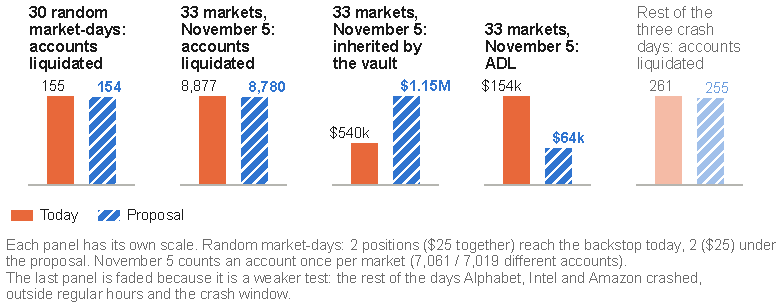
\includegraphics[width=.8\textwidth]{figs/normal_days.pdf}\end{center}
\vspace{-1.5ex}

\par{\small\color{mute}Sources: random sample, drawn with a fixed seed (the nine days used elsewhere excluded); 33 markets and the crash days: \S\ref{sec:three}, page~\pageref{sec:three}. Rules we tested and dropped because traders would have felt them (lower leverage for large positions, a leverage cut around earnings, earlier liquidation for everyone): the companion note on earlier variants.\par}

%======================================================================================== 16 attackers
\page{Test results: a wrong price alone moves the mark slowly; a walked price with a book push does as much harm as today, or more}{What was tested \,·\, condition 2: attacks should do less harm}\phantomsection\label{sec:attacks}

Every attack we designed on xyz's pricing rules was replayed under today's rules and under the proposal, through real accounts with real margin that can be liquidated like anyone else. Taken one at a time, a short wrong price, a walked external price and a push of xyz's book while the feed and the anchor agree were each outvoted in the tests, on deep and thin books alike; when they are apart, as during a real move, a push sets the mark between them (page~\pageref{sec:vote}).

\begin{center}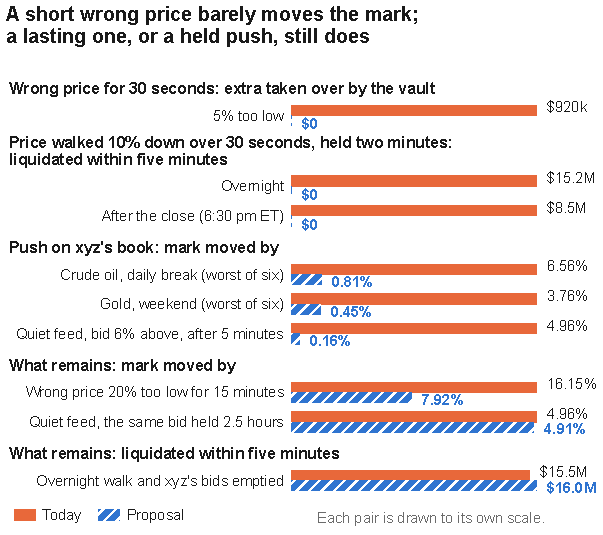
\includegraphics[width=.6\textwidth]{figs/attacks.pdf}\end{center}
\vspace{-1.5ex}

\textbf{What the proposal leaves open.} Someone who walks the external price and empties one side of xyz's book gets two votes to agree: on Alphabet overnight \$15.5M is liquidated today and \$16.0M under the proposal (\$15.2M today with the walk alone). Selling into every bid within 10\% of the price takes well under \$1.5M of margin on every market we measured:

{\small
\begin{tabularx}{\textwidth}{@{}>{\raggedright\arraybackslash}Xrr@{}}
\toprule
Typical minute, on the days replayed & Bids within 10\% of the price & Margin needed to take them all\\
\midrule
Reddit, overnight (the least) & \$280k & \$30k\\
Alphabet, overnight & \$6.14M & \$310k\\
SK Hynix, Korean trading hours (the most margin) & \$12.24M & \$1.22M\\
\bottomrule
\end{tabularx}}

So this attack stays open; we think the protection lies in the quality of the external price (change 6). The correction step is not what makes it succeed: without it these tests give the same figures. A push of the book kept up for hours while the feed is not live also still moves the mark, about 2\% per hour (change 2).

\foot
\begin{exact}[Sources]
Margin $=$ bids $/$ maximum leverage, median minute of the book rebuilt on 22 market-days, market makers assumed not to refill (a lower bound on the cost). Every test, with every walk: \S\ref{sec:three}, page~\pageref{sec:three}. Closures: \S\ref{sec:closed}. A remark for Hyperliquid, outside the six changes, on a book with one side empty (ENA, a token on another Hyperliquid exchange, March 14, 2026): \S\ref{sec:three}, page~\pageref{sec:three}. Earlier rules against a walked feed, all rejected: the companion note on earlier variants.
\end{exact}

%======================================================================================== 17 costs
\page{What it costs: where the suggestions do worse than today, do no better, or were not tested}{The other side of the ledger \,·\, each figure today first, then the proposal (changes 1 to 3 together)}\phantomsection\label{sec:costs}

{\small
This page gathers every test where the proposal does worse than today, no better, or was not tested (figures: \S\ref{sec:three}, page~\pageref{sec:three}). \textbf{The pattern.} In most tests the vault inherits more under the proposal than today: Alphabet's earnings crash, SK Hynix on July 27, the 33 markets of November 5, five market-days held out of the design, a stuck feed, a frozen book and the 23 largest positions. It inherits less on Intel, on Amazon within the replay's error, and on the two oil markets of September 10. By page~2's ranking, more inherited matters through the money to avoid ADL and capital given beside it below: on the three crashes together both fall (\$462k, \$352k; \$715k, \$589k), on Alphabet both rise. The replay favors the proposal in one known way, the read lag (page~\pageref{sec:limits}).

\textbf{Worse than today.}
\begin{itemize}[leftmargin=1.3em,itemsep=0pt,topsep=0pt,parsep=0pt]
\item \textbf{A walked external price with a push of xyz's book} (page~\pageref{sec:attacks}): Alphabet overnight \$15.5M liquidated, \$16.0M; after an upward walk after the close \$1.01M, \$2.64M; a downward one with a 60-second push \$12.1M, \$12.6M; Amazon and Intel up to \$1.94M, \$1.99M. \textbf{A downward push held an hour} on a feed that is not live: 0.97\%, 2.10\%; after any push the proposal's mark returns more slowly.
\item \textbf{The mark above the book for hours} (change 2, page~\pageref{sec:skhx}): on SK Hynix, July 27, between 11:00 and 23:00 today's mark stayed within 0.93\% of the book; the proposal's was more than 2\% above it on 20.9\% of updates, more than 5\% on 3.2\%, at most 7.03\%. Whether a trader could draw value from it, and its effect on funding, were not tested.
\item \textbf{Earnings crashes} (page~\pageref{sec:res-mark}), \textbf{Alphabet:} inherited \$6.96M, \$10.28M; capital \$329k, \$419k; money to avoid ADL \$185k, \$219k. Three crashes: inherited \$10.75M, \$11.90M. \textbf{A \$1M push during the crash:} capital \$771k, \$863k (the gap is Alphabet's). \textbf{External price frozen two minutes:} capital \$939k, \$974k; inherited \$15.11M, \$18.48M. \textbf{xyz's whole book standing still five minutes} (Alphabet): mark up to 4.78\% above the external price, 8.65\%; 217 takeovers (197 below the external price), 331 (306); inherited \$11.41M, \$16.26M; capital \$498k, \$540k; money to avoid ADL \$280k, \$286k; value at takeover (their worth at the external price when handed over, not the vault's result) $-\$44.8$k, $-\$210.7$k.
\item \textbf{SK Hynix, July 27} (pages~\pageref{sec:skhx}--\pageref{sec:skhx2}): 352 takeovers (349 below the external price), 595 (586); inherited \$15.90M, \$19.05M; value at takeover $-\$1.79$M, $-\$2.45$M (not the vault's result). Money to avoid ADL falls 38\% (\$1.43M today, \$892k), but that rests on xyz's book stopping at 955, the edge of today's bound around the wrong price 868.18; had the book followed that price, the proposal's mark could have gone below today's low of 917. The result is indeterminate.
\item \textbf{November 5, 33 markets} (page~\pageref{sec:users}): inherited \$540k, \$1.15M (about \$30k against \$640k without the false takeover); capital \$0, \$8k; ADL and inherited together about \$184k, \$704k. \textbf{Five other market-days held out of the design} (page~\pageref{sec:res-mark}): takeovers 8, 11; \$5k, \$100k; the seven together need under \$50, about \$100 to avoid ADL. \textbf{The 23 largest positions of the crashes} (page~\pageref{sec:res-cut}): \$8.72M, \$9.78M.
\item \textbf{Sales of large positions} (change 3, page~\pageref{sec:res-cut}): median sale \$47k, \$77k; filled 0.62\% below the external price, 1.29\%; the worst tenth take 26\% of the book within 1\% of the best price, 36\%, and move the best price 0.50\%, 0.73\%.
\item \textbf{More stop orders fire on Amazon's crash day} (page~\pageref{sec:users}): 295, 390.
\item \textbf{Funding} (change 1): while the feed is live the oracle is the raw external price, without today's 0.5\% clamp, so a wrong print reaches funding in full; probably small, not replayed (page~\pageref{sec:limits}).
\end{itemize}
\textbf{No better than today, or a change to documented behavior.}
\begin{itemize}[leftmargin=1.3em,itemsep=0pt,topsep=0pt,parsep=0pt]
\item \textbf{Random market-days:} the mark is a median 0.03\% from today's, but on the worst one more than 1.6\% away for 1\% of the time (page~\pageref{sec:users}).
\item \textbf{A lasting wrong external price} (page~\pageref{sec:attacks}) still moves the mark and liquidates healthy accounts: after 15 minutes of a 20\% error, 16\% and 801 accounts today, 7.92\% and 559. With a \$5M push as well, the mark moves at most 16.15\% today, 13.10\%; more is liquidated through the book under the proposal (\$3.09M, \$6.04M), while the total liquidated is lower (\$25.3M, \$18.2M). \textbf{One wrong price followed by no change} starts the internal price (not measured).
\item \textbf{Change 2's 1\% cap} (page~\pageref{sec:notlive}; figures \S\ref{sec:closed}, page~\pageref{sec:closed}): on 510 closures the mean gap at reopening is 0.477\% today, 0.478\%, and two closures end more than 0.5\% further from the reopening price than today. \textbf{No resets under change 2:} as written, discovery in a closed session is limited to $1/\text{maxLev}$ around the last external price; trade.xyz's resets (re-anchoring the band near its edge) could be kept; untested either way. \textbf{The anchor is exempt from the discovery bound} (page~\pageref{sec:vote}), so the mark can leave it (how often was not measured); trade.xyz documents that a position whose liquidation price is outside the bounds cannot be liquidated, and the proposal would change that documented behavior.
\item \textbf{Change 4}, six more markets for the vault, would not have prevented past ADL (page~\pageref{sec:ceiling}); 92 isolated-only markets keep ADL. The vault's capital for its six markets was not computed. Its switch is irreversible, can lead to a review of trade.xyz's stake, and moves all of a cross account's positions to the vault at a takeover.
\end{itemize}
\textbf{Not tested.} Change 6, the items for the external price (no test shows they stop a walk); whether, on July 27, the book would have gone below 955 under the proposal; change 1 with today's internal price; the switching of change 2 on its own; a relayer restart; a feed flickering by one tick; halts over two minutes; splits, dividends and rolls.\par}



%======================================================================================== 17b limits
\page{What the study cannot tell: today's rules are reconstructed, the days are few, and the book does not react}{The limits of every result in this paper}\phantomsection\label{sec:limits}

What follows limits every result in this paper: how the replay was built, which days it covers, and what it cannot see.
\begin{itemize}[leftmargin=1.3em,itemsep=.6ex,topsep=0pt]
\item \textbf{Today's rules are our reconstruction:} it includes a read lag (the delay with which today's relayer reads the external price, as we reconstruct it) and corrections fitted to the chain record. The proposal is replayed as written, with neither. The read lag delays today's mark, so in fast crashes it favors the proposal; we have not measured by how much.
\item \textbf{The replay is not exact.} On November 5 it shows a \$510k takeover that never happened on the chain. A gap as small as Amazon's capital need, \$143k today against \$125k under the proposal, should not be read as a gain.
\item \textbf{Two simplifications favor one side.} The book's mid stands in for trade.xyz's documented impact price, so today's closed-market pushes may be overstated. The replay has no re-anchoring of the discovery bound (``resets'') under either rule set.
\item \textbf{The tests are a handful of hard days,} and the formula was chosen after about forty variants tried on them, mostly other mark formulas, margin rules and liquidation sizes (the companion note); only the random sample was untouched, and two of its drawn days, which could not be rebuilt, were replaced by reserves. Why we expect the result to hold beyond them, and what would test it: page~\pageref{sec:tests}.
\item \textbf{Funding is not replayed}, so the effect of a raw external price on funding (page~\pageref{sec:costs}) is not measured.
\item \textbf{The order book does not react.} Every replay uses the book as recorded; how market makers would react, and the vault's profit or loss when it sells, are not measured.
\item \textbf{The specification that accompanies this paper (page~\pageref{sec:tests}) leaves open} what a live relayer can read in time, how it restarts, how several relayer instances share the anchor's state, and how the anchor is rounded (off the price grid in the replay). Its test day, July 27, does not exercise the internal price's bound, a one-sided book or a restart.
\item \textbf{The capital figures are estimates} on 209 days of hourly prices, with an instant move (page~\pageref{sec:capital} and \S\ref{sec:cover}).
\end{itemize}

\par{\small\color{mute}Sources: every test, \S\ref{sec:three}, page~\pageref{sec:three}; the capital estimates, \S\ref{sec:cover}.\par}


\clearpage}

%==========================================================================================
\clearpage
\setlength{\parskip}{.35ex}
\appendix
{\LARGE\bfseries Appendix: today's rules and the proposal in full\par}\vspace{1.5ex}

\noindent Terms in \textcolor[HTML]{2F74D0}{\textbf{blue}} are what the proposal changes against today's rules. The variants we tried before the proposal, and the earlier runs that scored them, are in a separate note, \emph{Variants tested before the proposal}; the paper states, where it uses them, what it takes from that note. Every figure here is from the final run unless a line says otherwise.

\phantomsection\label{sec:appintro}\textbf{How to read the results.} Every result comes from the replay engine of page~\pageref{sec:tests}; in the final run its mark equals the chain's at these shares of the liquidation blocks of the seven held-out market-days: Brent oil 172 of 173, crude oil 177 of 177 (September 10), gold 195 of 199, SpaceX 79 of 80 (October 30), Alphabet 72 of 73, Meta 138 of 139, silver 133 of 133 (October 22); on the five isolated-only ADL days, measured on the rebuild of November 11, at 162 of 165 (ServiceNow 29 of 30, Lumentum 31 of 31, Marvell 17 of 17, Reddit 44 of 44, Cloudflare 41 of 43). Unless a line says otherwise, it is the total over the three earnings crashes (Alphabet on October 28, Intel and Amazon on October 29), and it is compared with today's rules on the same days. The words used:
\begin{itemize}[leftmargin=1.2em,itemsep=0pt,topsep=.2ex]
\item \emph{Takeovers} and \emph{inherited}: how many positions the vault takes over, and their total size in dollars.
\item \emph{Value at takeover}: what those positions were worth, at the external price, at the moment the vault took them, summed. Negative means the positions were already worth less than zero when taken; positive means they still had margin left. It is not the vault's profit or loss, which depends on how it later sells them and is never reported.
\item \emph{Below the external price}: takeovers already worth less than zero when taken.
\item \emph{Stops fired}, \emph{accounts hurt}: stop orders triggered, or accounts liquidated, that would not have been without the test's disturbance.
\item \emph{Wrong price}: the external price off by $-5\%$ for 30\,s, or by $-20\%$ for 2, 5 or 15\,min, at 6:30\,pm ET on Alphabet and Amazon. \emph{Stuck feed}: the external price frozen for 2\,min as the crash begins. \emph{Walk}: the external price moved 10\% away step by step.
\item \emph{Hold}: a second rule of earlier candidates, left out of the proposal: while xyz's book and the feed disagree, the center of the discovery bound stays where it was.
\item \emph{Final run}: our last replay of every test, on the market-days as rebuilt, with the proposal as written (no hold); \emph{earlier run}: a replay on the days as first built, before the rebuild. \emph{Scorecard}: the table of every test in the final run (\S\ref{sec:three}). \emph{Correction step}: each update, the anchor is pulled back between the feed's vote and the last mark (change 1). \emph{Cut-back}: change 3, sales that restore initial margin.
\item \emph{Held out}: seven market-days held out from the first designs; the oil days among them later shaped change 2 (\S\ref{sec:three}, \S\ref{sec:closed}).
\end{itemize}
trade.xyz changed parameters within the 392 days, among others the internal time constant (8\,h to 1\,h on November 21, 2025; 30\,min on April 30, 2026), the discovery bound's re-anchoring (March 13), more resets on nearly every market together with higher leverage and tighter bounds on five of them (June 12), and resets on seven further markets (October 25). The data windows differ by source: the record of fills covers 392 days, hourly prices 209 days (the capital study), the random sample was drawn from July 1 to November 8 (the days used fall between August 4 and October 1), and the feed study used four days. Today's rules are our reconstruction; two rules found on the chain record were added to it on November 8: the first mark input is clamped around the previous mark on the chain, not around the oracle; and in the futures' daily break and on weekends the oracle is trade.xyz's internal price, a 30-minute average of xyz's book (\S\ref{sec:current}).

\section*{Notation}
\begin{xltabular}{\textwidth}{@{}>{\raggedright\arraybackslash}p{5.6cm}X@{}}
$t$ & relayer update (one price update by trade.xyz, every $\approx 3$\,s); $k\ge1$ its read lag\\
$E_t$ & trade.xyz's external price (the asset's own market)\\
$B_t = \med(\text{bid}_t,\text{ask}_t,\text{last}_t)$ & xyz book price, computed by Hyperliquid\\
$O_t$;\ $X^1_t, X^2_t$ & oracle; the two mark inputs trade.xyz publishes\\
$M_t$ & mark price\\
$c$ & 0.5\%, the relayer's clamp per update\\
$d$ & $1/\text{maxLev}$ for most markets; trade.xyz re-anchors the bound's reference when the price nears its edge, a set number of times per direction (``resets''), which our replay does not model, for today's rules or the proposal\\
$\D_t(x) = \clip\big(x,[R_t(1-d),R_t(1+d)]\big)$ & discovery bound, center $R_t = E_t$ unless stated\\
$e_t = \ema_{150\,\text{s}}(\text{mid}-E)$ & premium average, sampled every 500\,ms\\
MM, IM & maintenance $=\tfrac12$ initial margin at max leverage\\
$V_t$, $A_t$, $\tilde A_t$ & the proposal: feed's vote, anchor, anchor before its correction step\\
$\kappa$, $\tau$ & 1\% cap on the internal price's pull toward the book; 30\,min averaging time\\
$\Delta t$, $\Delta t^*$ & time since the previous update; $\min(\Delta t, \tau/10)$\\
mid, $E_{\text{last}}$ & midpoint of xyz's best bid and ask; latest external price received\\
hull$[a,b]$, $H_t$ & the range spanned by two intervals; today's second-input clamp\\
$[a,b]$ & the range between $a$ and $b$, whichever is larger\\
$q$, $q_{\text{left}}$ & position size; size left after a sale\\
eq$'$, MM$'$, $r_m$ & equity and maintenance margin after a move; the move of market $m$\\
$\mathcal{P}$, $C$ & the set of open positions; the vault capital for them
\end{xltabular}

%==========================================================================================
\section{Today's rules}\label{sec:current}
As we reconstruct them from the chain record. trade.xyz's documentation gives the median of three inputs, the 150\,s average and the 0.5\% clamp per update; the read lag $k$, the first input's clip to the previous mark, the hull clamp, the 500\,ms sampling and the bound on the oracle and inputs are what the chain shows.

\textbf{Relayer (trade.xyz), external session.}
\begin{align}
O_t &= \D_t\big(\clip(E_t,\ O_{t-k}(1\pm c))\big)\\
X^1_t &= \D_t\big(\clip(O_t,\ M_{t-1}(1\pm c))\big) \label{eq:x1}\\
X^2_t &= \D_t\big(\clip(E_t + e_t,\ \text{hull}[\,O_{t-k}(1\pm c),\ X^2_{t-k}(1\pm c)\,])\big)
\end{align}
\textbf{Relayer, closed market} (as on the tested days: the futures daily break, 5 to 6\,pm ET; weekends; Korean closed hours, now 8:00\,pm to 9:01\,am and 3:20 to 4:05\,pm KST; and after a data gap of 15\,s for Korean stocks or 30\,s for FX): the internal price, an average of xyz's own book (the mid stands in for the documented impact price, which does not move while the price sits between the impact bid and ask and ignores a thin side, so today's closed-market push figures may be overstated),
\begin{equation}
O_t = O_{t-1} + \big(1 - e^{-\Delta t^*/\tau}\big)\,(\text{mid}_t - O_{t-1}),\qquad \tau = 30\,\text{min},\ \ \Delta t^* = \min(\Delta t, \tau/10)
\end{equation}
\textbf{Hyperliquid.} $M_t = \clip\big(\med(X^1_t, X^2_t, B_t),\ M_{t-1}(1\pm1\%)\big)$; with the relayer silent 10\,s, $M_t = B_t$.
Liquidation: below MM, market orders (positions over \$100k: a first order for 20\%, then full-size orders during a 30\,s cooldown, from Hyperliquid's documentation; trade.xyz's page describes full-size orders); below $\tfrac23$MM the backstop vault takes the position, in our replay at the bankruptcy price; ADL last: on isolated-only markets the book keeps selling below $\tfrac23$MM, and the position is auto-deleveraged once its equity is negative (as documented), in our replay at the previous update's mark, as the chain shows.
\res{Final run, on the market-days as rebuilt: on the three crashes \$10.75M inherited, 814 of 819 takeovers below the external price, value at takeover $-\$157.9$k (not the vault's result); with a stuck feed \$15.11M; on the seven market-days 103 takeovers and \$1.25M; a wrong price of $-5\%$ for 30\,s at 6:30\,pm ET on Alphabet hands the vault \$920k of healthy positions.}

%==========================================================================================
\section{The proposal}\label{sec:three}
\par{\small\color{mute}Who would ship it: relayer + Hyperliquid (the cut-back).}\par
One formula replaces today's rule of following $E$ at 0.5\% per update, and every earlier hold: the mark is the median of three votes, the feed, xyz's book and a 30-minute average of the feed (the anchor).
\begin{align}
O_t &= \chg{\D_t(E_t)}\quad\text{(feed live)},\qquad \chg{V_t = E_t \text{ if the feed is live, else } O_t}\\
\tilde A_t &= \chg{A_{t-1} + \big(1 - e^{-\Delta t/\tau}\big)(V_t - A_{t-1})},\qquad \tau = 30\,\text{min},\ A_0 = E_0\\
A_t &= \chg{\tilde A_t}\ \text{ if } B_{t-1} \text{ was strictly between } V_{t-1} \text{ and } A_{t-1},\ \text{ else }\ \chg{\clip\big(\tilde A_t,\ [V_t, M_{t-1}]\big)}\\
M_t &= \clip\big(\med(\chg{V_t},\ \chg{A_t},\ B_t),\ M_{t-1}(1\pm 1\%)\big)
\end{align}
\textbf{Feed live or not.} Feed live: the venue is open and $E$ changed in at least one of the last two updates. Feed not live (closure, or $E_t = E_{t-1} = E_{t-2}$): the capped internal price of \S\ref{sec:closed}, $\kappa = 1\%$, kept within the discovery bound of the last external price ($O_t \in E_{\text{last}}(1\pm d)$), with the same mark formula; the anchor keeps running and is never restarted.

\textbf{How often.} On six replayed market-days the external price is unchanged on 6 to 27\% of updates in regular hours and 39 to 87\% overnight; the rule is on for 0.6 to 8.9\% of updates in regular hours (switching on 7 to 70 times an hour, spells of 3 to 5\,s) and 20 to 79\% overnight (36 to 90 times an hour, spells of 7 to 36\,s). In a spell of one or two updates the internal price moves at most about 0.002\% per update, unless the external price has just jumped (it then restarts from the new value, as on July 27); the effect of the switching was not replayed on its own.

\textbf{Inputs.} The relayer publishes $V$ and $A$ as its two mark inputs; Hyperliquid's formula is unchanged. Inputs at update $t$: the current external price $E_t$ (or $O_t$) for $V_t$; for $A_t$, the previous $A_{t-1}$, $V_{t-1}$, $B_{t-1}$ and $M_{t-1}$. In the replay these are the previous update's published values exactly; what a live relayer can read in time, and how it restarts, is left to the implementer (the specification lists both as open). 

\textbf{Correction step.} The anchor is kept between the feed's vote and the previous mark, unless xyz's book lay strictly between the vote and the anchor at the previous update, when it can lag (Alphabet crash: 13 updates, up to 3.66\% above the mark); it does not follow a previous mark that xyz's book alone decided while the book is still pushed. When the book comes back after a dip during a lasting wrong price, though, the mark can rise only 1\% per update and the correction step pulls the average down to it, so part of the dip stays (worst case below). It is exempt from the discovery bound; since the median lies between $V_t$ and $A_t$, the mark can then leave the bound while the anchor is outside it.

\textbf{Rounding and the specification.} We suggest the relayer keep the internal price unrounded and publish it rounded (stepping from the rounded price stalled it on SK Hynix in the engine, tick 0.1). From the specification: on entering a closure the internal price starts from the price published at the update before; a change of $E$ inside a closure only moves the bound $E(1\pm d)$ and does not restart it; with one side of the book empty the book price is the lone quote and the internal price keeps the last mid seen with both sides; $A$ is published to the nearest $10^{-6}$ USD, off the price grid; when $V_{t-1} = A_{t-1}$ the ``strictly between'' test is false, so the clip applies. Liquidation: the cut-back above \$100k (page~\pageref{sec:cutback}).

\textbf{For an implementer.} The specification lists two decisions needed first: whether the anchor may be published off the price grid (it is in the replay, on 14{,}675 of 29{,}010 updates), and which rounding Hyperliquid's 1\% limit uses. A restarted relayer would publish $A = V$, so the mark becomes $V$ on that update unless $A$ is stored. With both sides of the book empty, or no trade yet, there is no book price and no mark at that update. The test vector of July 27 exercises 17{,}322 updates that are not live, 733 starts of the internal price and the correction step; it does not exercise the bound $E(1\pm d)$, the 180\,s cap on the time step, an empty side of the book, a read delay or a restart.
\res{Final run of November 13, 2026 on the 22 rebuilt market-days of the table below (the 33-market day and the 30 random market-days were built separately). The earlier candidates' \$0, or no cascade, on July 27 (details in the companion note on earlier variants) came from their hold; every proposal figure here is without it (why it is left out: the item on the hold below).\par
{\footnotesize\renewcommand{\arraystretch}{1.0}\begin{xltabular}{\textwidth}{@{}>{\raggedright\arraybackslash\hangindent=1em\hangafter=1}Xrr@{}}
\toprule
Test & Today & Proposal\\
\midrule
\endhead
Three crashes: capital the vault needs & \$715k & \$589k\\
Three crashes: money the vault needs to avoid ADL & \$462k & \$352k\\
Three crashes: inherited by the vault & \$10.75M & \$11.90M\\
\quad Alphabet, October 28: capital need & \$329k & \$419k\\
\quad Alphabet: money to avoid ADL & \$185k & \$219k\\
\quad Alphabet: inherited & \$6.96M & \$10.28M\\
\quad Intel, October 29: capital need & \$244k & \$45k\\
\quad Intel: money to avoid ADL & \$166k & \$33k\\
\quad Intel: inherited & \$2.24M & \$300k\\
\quad Amazon, October 29: capital need & \$143k & \$125k\\
\quad Amazon: money to avoid ADL & \$112k & \$99k\\
\quad Amazon: inherited & \$1.55M & \$1.32M\\
SK Hynix, July 27: capital need & \$2.60M & \$2.27M\\
SK Hynix: money to avoid ADL & \$1.43M & \$892k\\
\quad today's mark with the cut-back; the proposal's mark with today's sizing & \$1.356M & \$883k\\
\quad inherited & \$15.90M & \$19.05M\\
\quad takeovers & 352 & 595\\
Five isolated-only replays: ADL & \$300.4k & \$99.5k\\
Seven other market-days: takeovers on two oil markets, September 10 (later shaped change 2) & 95 & 13\\
\quad on the five other market-days (Alphabet, Meta, silver, gold, SpaceX) & 8 & 11\\
\quad all seven & 103 & 24\\
\quad inherited & \$1.25M & \$180k\\
\quad capital need & \$24.5k & \$900\\
\quad money to avoid ADL & under \$50 & \$100\\
\bottomrule
Feed stuck 120\,s at the crash onset: capital need & \$939k & \$974k\\
\quad money to avoid ADL & \$590k & \$559k\\
Wrong price $-5\%$ for 30\,s (Alphabet, 6:30\,pm ET; the other two tests: \$200k and \$0 today, \$0 proposal): healthy positions taken over & \$920k & \$0\\
Wrong price $-20\%$ for 2 / 5 / 15\,min (Alphabet, 6:30\,pm ET): largest mark move by then & 16.14 / 16.15 / 16.15\% & 1.35 / 2.92 / 7.92\%\\
\quad extra taken over by the vault & \$7.40M / \$7.41M / \$7.49M & \$0 / \$0 / \$0\\
\quad extra liquidated through the book & \$13.47M / \$13.56M / \$14.11M & \$0 / \$2.94M / \$10.82M\\
\quad accounts liquidated through the book & 790 / 797 / 801 & 0 / 150 / 559\\
Worst case: wrong price $-20\%$ for 15\,min and a 45\,s \$5M push of the book 10\% down: mark moved after 2 / 5 / 15\,min & 16.14 / 16.15 / 16.11\% & 9.32 / 10.15 / 13.10\%\\
\quad extra liquidated through the book; extra to the vault & \$3.09M (625); \$22.17M (715) & \$6.04M (587); \$12.15M (784)\\
\quad the same with \$1M of attacker capital: mark moved after 2 / 5 / 15\,min (under the proposal the attacker runs out of margin before the book dips) & 16.14 / 16.15 / 16.11\% & 1.34 / 2.92 / 7.92\%\\
Walk $-10\%$, Alphabet overnight: liquidated in 5\,min & \$15.2M & \$0\\
\quad the same after the close (6:30\,pm\,ET) & \$8.5M & \$0\\
\quad the same on SK Hynix, July 27, 03:00 UTC & \$9.4M & \$0\\
Overnight walk and a \$1M book push over 15\,s: liquidated in 5\,min & \$15.1M & \$14.0M\\
\quad push over 60\,s & \$15.5M & \$16.0M\\
After-close walk and a \$5M book push over 15\,s: liquidated in 5\,min & \$11.0M & \$3.1M\\
\quad push over 60\,s & \$12.1M & \$12.6M\\
After-close walk $+10\%$ and a \$5M push over 15 / 60\,s: liquidated in 5\,min & \$370k / \$1.01M & \$180k / \$2.64M\\
Overnight walk $+10\%$ and a \$1M push over 15 / 60\,s & \$310k / \$430k & \$150k / \$410k\\
Amazon, Intel, overnight and after the close, walks of $\pm10\%$ with a push & \$50k to \$1.94M & \$30k to \$1.99M\\
Closed crude oil / gold, worst push: taken over beyond the same day without a push & \$5.47M / \$40k & \$340k / \$0\\
Closed crude oil, book pushed 1 to 15\,min: mark lift & 2.11--6.56\% & 0.10--0.81\%\\
Closed gold, book pushed 1 to 15\,min: mark lift & 1.96--3.76\% & 0.03--0.45\%\\
Quiet feed, \$5M bid 6\% above: mark lift after 5\,min & 4.96\% & 0.16\%\\
\quad after 1\,h & 4.70\% & 1.86\%\\
\quad after 2.5\,h & 4.96\% & 4.91\%\\
Quiet feed, \$5M push 6\% below: mark move after 5\,min / 1\,h / 2.5\,h (as measured; the path is not monotone) & 1.47 / 0.97 / 1.49\% & 0.17 / 2.10 / 1.23\%\\
Crash, \$5M book push over 60\,s: capital need (the attacker loses all) & \$899k & \$802k\\
\quad push over 300\,s & \$899k & \$840k\\
Crash, \$1M book push over 60 or 300\,s: capital need (without a push: \$329k / \$419k) & \$771k & \$863k\\
Rest of the crash days, outside regular hours and the crash window: accounts liquidated, Alphabet & 184 & 180\\
\quad Intel & 56 & 55\\
\quad Amazon & 21 & 20\\
23 largest positions of the crashes: inherited by the vault & \$8.72M & \$9.78M\\
November 5, 33 markets: accounts liquidated & 8{,}877 & 8{,}780\\
\quad ADL on isolated-only markets & \$154k & \$64k\\
\quad inherited by the vault & \$540k & \$1.15M\\
\quad capital need & \$0 & \$8k\\
\bottomrule
\end{xltabular}}\par
{\footnotesize The push down and the push up on a quiet feed differ under both sets of rules (today 1.47\% against 4.96\% after five minutes; under the proposal 1.23\% against 4.91\% after 2.5\,h, and 2.10\% against 1.86\% after an hour). One side of xyz's book may simply absorb \$5M more than the other.\par}
\begin{itemize}[leftmargin=1.2em,itemsep=.2ex,topsep=.3ex]
\item \textbf{Rest of the crash days} (outside regular hours and the crash window). The mark sits a median 0.008 to 0.010\% from today's; on Amazon one account is liquidated under the proposal only and two under today's rules only (21 today, 20). Stops fired outside regular hours, today against the proposal: Alphabet 763 against 710, Intel 1{,}398 against 1{,}387, Amazon 295 against 390; fired under the proposal only: 49, 9 and 146.
\item \textbf{By combination.} ADL on the five isolated-only replays (Cloudflare on November 5 among them): today \$300.4k, cut-back alone \$301.1k, the proposal's mark alone \$135.3k, the proposal \$99.5k. The 23 largest positions, inherited by the vault: today's mark with today's sizing \$8.72M, with the cut-back \$9.32M; the proposal's mark with today's sizing \$11.76M, with the cut-back \$9.78M.
\item \textbf{November 5.} \$510k of the \$540k simulated under today's rules is one S\&P 500 takeover that did not happen on the chain, the same under every rule. On the chain that day the backstop events came to \$154k, all ADL on isolated-only markets: Cloudflare \$137.0k, DraftKings \$9.1k and two smaller markets (\$8.3k and \$28), the 25 ADL events of the record of fills (\S\ref{sec:cover}); the replay of today's rules gives \$154k of ADL on the same markets (Cloudflare \$134k, DraftKings \$10k, \$8k on the first of the two smaller markets, and under \$1k on three others), within \$3k market by market: agreement with the chain, from 38 replayed events against 25 recorded ones. The vault itself took nothing on the chain that day.
\needspace{16\baselineskip}\item \textbf{The correction step, with and without} (every final test replayed without it; today / proposal / without the step):\par
{\footnotesize\begin{tabularx}{\linewidth}{@{}>{\raggedright\arraybackslash}Xrrr@{}}
\toprule
Test & Today & Proposal & Without the step\\
\midrule
Worst case (20\% wrong price 15\,min, 45\,s \$5M push): mark moved after 2 / 15\,min & 16.14 / 16.11\% & 9.32 / 13.10\% & 1.57 / 8.15\%\\
Book push during the Alphabet crash, \$5M for 300\,s: capital need & \$899k & \$840k & \$1.188M\\
\quad the same for 60\,s & \$899k & \$802k & \$825k\\
Overnight walk $-10\%$ then a \$1M push: liquidated in 5\,min, walk / +15\,s / +60\,s & \$15.23M / \$15.10M / \$15.52M & \$0 / \$14.03M / \$16.02M & \$0 / \$13.96M / \$16.01M\\
After-close walk $-10\%$ then a \$5M push: the same & \$8.54M / \$10.97M / \$12.09M & \$0 / \$3.06M / \$12.61M & \$0 / \$3.49M / \$12.62M\\
Wrong price 5\% low for 30\,s: mark moved & 4.17\% & 0.10\% & 0.50\%\\
Wrong price 20\% low, 15\,min, alone: mark moved at 15\,min & 16.11\% & 7.92\% & 8.15\%\\
Whole book frozen 5\,min: largest gap / inherited & 4.78\% / \$11.41M & 8.65\% / \$16.26M & 7.84\% / \$14.78M\\
Feed stuck 120\,s at the crash onset: capital need / inherited & \$939k / \$15.11M & \$974k / \$18.48M & \$926k / \$16.73M\\
Three crashes, SK Hynix, isolated-only replays, held-out days, closed-market pushes & \multicolumn{3}{r}{the two versions agree closely (inherited within about \$160k)}\\
\bottomrule
\end{tabularx}}\par
Each version has tests where it is the worse one. With the step the proposal is worse than today with a stuck feed (\$939k today, \$974k) and a frozen book; without it, the crash push is worse than today (\$899k today, \$1.188M), and so is the frozen book. The worst case of a wrong price with a book dip is better without the step (13.10\% with it, 8.15\% without), and the walk-plus-push tests are the same either way.
\item \textbf{The hold, left out.} Several earlier candidates (details in the companion note on earlier variants) need \$0, or start no cascade, on July 27: that came from a hold, a second rule that freezes the price band when the feed and xyz disagree. We left it out. It has three constants of its own (a disagreement threshold, a step every 150 seconds, a size for reading the book); it depends on reading xyz's recent trades and book depth, which the design avoids; and one formula is easier to check than two. Its price is July 27 (page~\pageref{sec:skhx2}): \$892k where the hold gave \$0 in replay. trade.xyz may weigh it differently.
\item \textbf{Value at takeover} (final run; not the vault's result). Three crashes: 814 of 819 takeovers below the external price today, 322 of 583 under the proposal; value at takeover $-\$157.9$k today, $+\$63.4$k (not the vault's result). Alphabet 156 of 158 against 12 of 258; Intel 258 of 258 against 23 of 29; Amazon 400 of 403 against 287 of 296. With today's mark and the cut-back: 838 of 845; with the proposal's mark and today's sizing: 322 of 580 (the same 322 as the proposal, a coincidence), so the change comes from the mark. SK Hynix, July 27: 349 of 352 against 586 of 595, $-\$1.79$M against $-\$2.45$M, doubtful because that day's reopening price is the bad one. Frozen book: 197 of 217 against 306 of 331, $-\$44.8$k against $-\$210.7$k. \textbf{Not in the final run:} accounts harmed in the closed-market pushes.
\item \textbf{Assumption.} The design assumes xyz's book follows a real move of $E$: if it did not, $V$ alone would move and the mark would follow at the anchor's pace, slower than today's 0.5\% per update. In the three crashes the book followed within a few updates. With the 20 largest makers (68\% of maker volume) removed for 5\,min at the Alphabet crash, the mark stayed within 1.57\% of $E$, as without the removal (today 4.78\%, 39\,s above 2\%). With the whole book frozen for five minutes from the onset (every order, change and cancel dropped; the external price falls as recorded), the proposal does worse than today: largest gap above $E$ 4.78\% today, 8.65\% under the proposal; back within 1\% after 314\,s under both (with the recorded book: 59\,s today, 11\,s under the proposal); 217 takeovers today, 331 under the proposal (197 and 306 of them below the external price), \$11.41M inherited today, \$16.26M, capital need \$498k today, \$540k, money to avoid ADL \$280k today, \$286k. One market, one crash, and a book nobody touches at all, takers included.
\item \textbf{The vault on Alphabet} carries more under this mark (capital need $+27\%$, inherited $+48\%$); the total gain comes from Intel.
\item \textbf{Not solved (a):} a walked feed \emph{and} an emptied bid side. Two votes agree and the mark follows (\$14 to 16M liquidated overnight, what today's rules lose to the walk alone). The book is no barrier: clearing the bids within 10\% of the mid takes \$30k (Reddit overnight) to \$1.2M (SK Hynix) of margin on the 22 market-days measured, \$30k to \$500k on US names overnight; we think the protection lies in the quality of $E$ (\S\ref{sec:erec}).
\item \textbf{Not solved (b):} a book push while the feed is not live moves the mark about 5\% in five minutes today, and about 2\% per hour under the proposal, in our replay never beyond $d = 1/\text{maxLev}$ (the replay has no bound resets). The crash book push is a vault stress case, not an attack that pays: the vault inherits the attacker's own position (\$29M) and no other account is liquidated by the push.
\item \textbf{One-sided books on the chain record.} With one side of the book empty, Hyperliquid's mark runs to the lone quote. ENA on another HIP-3 exchange, March 14, 2026, 07:08 UTC: no bids, one ask at 0.20, oracle 0.1076, mark from 0.1199 to 0.1392 in 54\,s, the mark 29\% above the oracle at 54\,s, and shorts liquidated and auto-deleveraged at fills up to 33\% above it at 54\,s and 40\% at 70\,s; seven more such events on other HIP-3 exchanges. An optional suggestion to Hyperliquid: a one-sided book does not vote.
\item \textbf{Random sample.} 30 market-days drawn at random (six days, five markets each, July 1 to November 8, fixed seed): two tiny takeovers (\$25 together) under both sets of rules, 155 against 154 accounts liquidated in the book; the mark's distance to today's is 0.034\% on the median market-day (0.137\% on the worst), and 0.17\% at the 99th percentile (1.6\% on the worst).
\end{itemize}}

%==========================================================================================
\section{Closed-market oracle}\label{sec:closed}
One rule for every scheduled closure (daily break, weekend, holiday). Holding the last external price is ruled out: on 510 real internal sessions (on the 109 markets that had a closure on the six days studied) it is the worst guess at reopen (mean gap 0.71\%, against 0.48\% for the internal price), and it would stop xyz discovering price over a weekend.

\subsection{Capped internal price}
\par{\small\color{mute}Who would ship it: relayer.}\par
The internal price's book input may sit at most $\kappa$ from the current oracle, so a push moves it at most $\approx\kappa/2$ in 15 minutes (traced on crude oil, from the push's start: in the pushed replay the proposal's mark rises 0.48\% in the 15 minutes, inside the cap; in the same replay without the push it falls 0.32\%, because the internal price follows the real book down; the 0.81\% quoted elsewhere is the distance between the two):
\begin{equation}
O_t = O_{t-1} + \big(1 - e^{-\Delta t^*/\tau}\big)\,\chg{\clip\big(\text{mid}_t - O_{t-1},\ \pm\kappa\,O_{t-1}\big)}
\end{equation}
\res{Screen on the 510 sessions (reopen gap = distance from the oracle at the end of the closure to the first external price after it). The SK Hynix column is not a measure of accuracy: on July 27 the price really fell about 9\% over the closure, and this screen cannot tell whether the first external price it compares with is the bad reopening price of page~\pageref{sec:skhx}, so a larger gap there is not necessarily worse:\par\begin{tabular}{@{}lrrrr@{}}
\toprule
$\kappa$ & push, 15 min & mean reopen gap & $>0.5\%$ worse & SK Hynix gap\\
\midrule
none (today; the internal price alone) & $\approx 2.3\%$ & 0.477\% & -- & 1.11\%\\
0.5\% (trade.xyz's clamp) & 0.25\% & 0.489\% & 2 & 5.82\%\\
1\% (Hyperliquid's cap)$^*$ & 0.50\% & 0.478\% & 2 & 1.89\%\\
2\% & 1.00\% & 0.478\% & 0 & 1.11\%\\
\bottomrule
\end{tabular}\par
The rows without an asterisk are a screen of the internal price alone, without any mark rule. $^*$ The 1\% row's reopen gap comes from a screen with an earlier candidate's mark. The push column is the internal price alone; the mark moves further today (6.56\% on crude oil, page~\pageref{sec:notlive}) because its two other inputs follow the book.\par
Engine runs with the mark of an earlier candidate (details in the companion note on earlier variants): in these runs any cap stopped the closed-market push, though a push kept up for hours still moves the mark (\S\ref{sec:three}). Under today's mark the cap alone does not (final run, today / cap alone / proposal): crude oil closed, \$5M bid 6\% above for 15\,min, largest mark lift 6.56\% / 6.48\% / 0.81\%; with \$1M of attacker capital 6.56\% / 6.25\% / 0.23\%; gold 3.76\% / 3.76\% / 0.45\%; quiet feed, \$5M bid held 2.5\,h, 4.96\% / 4.96\% / 4.91\% at the end (0.16\% for the proposal after 5\,min); on the four recorded crashes the cap alone gives today's takeovers, capital need and money to avoid ADL (one takeover fewer on SK Hynix). Today's second input (the external price plus a 150\,s average of the book's distance from it) and the book itself follow the push whatever the internal price does, and the first input, kept within 0.5\% of the previous mark, is dragged along (5.43\% against 6.10\% without the cap). The cap protects only once the mark's inputs are the feed's vote and its average (change 1). With the earlier candidate's mark: crude oil's daily close, worst case 3 accounts hurt and the mark lifted 0.50\% (today, in that earlier run, 148 and 4.99\%; uncapped 55 and 2.16\%); gold weekend 0 accounts and 0.50 to 0.76\% (today, in that earlier run, 26 and 4.00\%; uncapped 17 and 2.59\%). With that earlier mark, the seven held-out market-days are unchanged under every cap. Chosen: 1\%, Hyperliquid's per-update mark cap, which tracks genuine moves on average as well as today at reopen (0.477\% today, 0.478\%; two sessions more than 0.5\% worse).}

%==========================================================================================
\section{Items for the external price \texorpdfstring{$E$}{E}}\label{sec:erec}
Any mark that follows $E$ follows a manipulated $E$, and handing the mark to xyz when they disagree hands it to whoever pushes xyz, which is cheaper. So we think the defense against a wrong $E$ lies in how trade.xyz builds it. From the chain record (the SOXL case below comes from an earlier pass over four days and the 126 markets that traded then; the rest matches page~\pageref{sec:feed}):
\begin{itemize}[nosep]
\item \textbf{Overnight, $E$ is often unchanged.} In the overnight session (for which trade.xyz's documentation names Blue Ocean ATS) $E$ is unchanged on 74.9\% of all updates taken together, on the 296 US market-nights of page~\pageref{sec:feed} (median market-night 78\%).
\item \textbf{One case where $E$ and xyz disagreed for long, and xyz was right.} SOXL (a leveraged semiconductor fund), October 21: $E$ frozen 2\,h at 104.77 while xyz traded down on real volume; $E$ resumed at 102.89.
\end{itemize}
trade.xyz's documentation says the relayer draws on several venues, markets and data providers, and names Blue Ocean ATS for the overnight session; how $E$ is computed and filtered is not documented, so what follows rests only on what the chain record shows. Suggestions to trade.xyz, all on its side (some may already be in place):
\begin{enumerate}[nosep]
\item \textbf{Publishing $E$'s age} (time since the source last traded or quoted) with every update, and stating what $E$ is built from in each session. The proposal treats an unchanged $E$ as not live; an explicit age makes that exact.
\item \textbf{Requiring a minimum size for what moves overnight $E$,} if that is not already the case. We do not know how $E$ is computed, so we cannot tell whether a small trade can move it today.
\item \textbf{Checking a move against the other sources $E$ draws on before publishing it,} if this is not already done, and holding a move that no other source confirms. We would not check it against xyz's book, which can be pushed, or a competitor's price, which we keep out of the design.
\end{enumerate}
Each one also shrinks one of the proposal's costs, a crash while the feed is frozen.

%==========================================================================================
\section{Backstop coverage and vault capital}\label{sec:cover}
\subsection{Isolated-only markets: the backstop is ADL}
\par{\small\color{mute}Who would ship it: trade.xyz.}\par
On a market whose margin mode forbids cross margin the vault cannot hold the position, so the backstop step is auto-deleveraging against profitable traders:
\begin{equation}
\begin{cases}\text{equity} < \tfrac23\,\text{MM}\ \Rightarrow\ \text{vault takes over} & \text{cross enabled}\\ \text{equity} < 0\ \Rightarrow\ \text{ADL at the previous update's mark} & \text{isolated-only (the book keeps selling until then)}\end{cases}
\end{equation}
Suggested: enabling cross margin on the isolated-only markets that clear the bar of page~\pageref{sec:five} (deployer action, irreversible; validators check liquidity, oracle and manipulation resilience, and a 50\% daily move triggers a review of the deployer's stake). The bar is the weakest of the 22 markets already cross-enabled on each criterion: a listed underlying; median daily volume on xyz over the 209 days of hourly prices at least Amazon's, \$8.0M; no 50\% day; no daily move larger than SanDisk's largest, 35\%. Clearing it: Robinhood, MicroStrategy, Nebius, AMD, the Korea fund EWY, Samsung (page~\pageref{sec:five}).
\resh{What the record of fills shows.}{The record of xyz fills (Hydromancer's archive), all 392 days (October 13, 2025 to November 8, 2026): 475 backstop events, 177 to the vault, 298 to ADL; \$85.2M of ADL. All of it but SK Hynix on July 27 (\$25.6M, the vault's balance was not enough) and silver on March 5 (\$1.5M, the day of the vault's first takeover there, when ADL fills still followed) came from markets before the vault's first takeover there: Brent oil \$33.3M (March 23), crude oil \$9.9M, silver \$550k (January 30), today's isolated-only markets \$13.45M (the Brazil fund EWZ \$9.34M, Unitree \$1.65M and others), and smaller amounts on other markets that have the vault today: \$58.1M in all. Apart from July 27 and March 5 (page~\pageref{sec:adl}), no market had ADL after the vault's first takeover there (switch dates are published only for five markets, on June 24; elsewhere the first takeover is our proxy): Brent oil last ADL March 23, first takeover May 23; crude oil last ADL May 24, published switch June 24, first takeover July 25; silver last ADL January 30, then March 5, the day of its first takeover. On November 5, the broadest selloff on record (median xyz market $-10\%$, 86 of 120 down more than 5\%), all 25 backstop events were ADL on isolated-only markets; the vault took nothing. In the engine, the four replayed isolated-only ADL days (ServiceNow, Lumentum, Marvell October 28; Reddit October 29; the mark is exact at 121 of 122 liquidation blocks on these four, and 41 of 43 on Cloudflare, November 5): in an earlier run ADL \$196k today (real \$171k), \$141k under an earlier candidate's mark (Marvell to \$0, Reddit halved; ServiceNow's earnings gap unchanged), \$0 with cross enabled (by construction: the vault takes the positions instead), where the vault would inherit the same positions. The isolated-only markets hold \$341M (17\%) of xyz's open interest. By status today: \$71.78M (84.2\%) of the ADL on record came from the 10 markets with ADL where the vault is allowed today, \$13.45M (15.8\%) from 34 still isolated-only, of which EWZ \$9.34M, Unitree \$1.65M and two others \$550k and \$530k; none of these clears the bar. The six markets of change 4 had \$20.7k in all (Samsung \$16.8k on May 25, 2026, Robinhood \$3.9k on February 10, 2026), so change 4 would have prevented almost none of the ADL on record; its case is forward-looking. The chart of page~\pageref{sec:ceiling} lands xyz's worst real 1-hour and 4-hour windows on the positions of October 30 at once, before any book liquidation, with and without the vault in the six markets: an upper bound, not an estimate.}

\subsection{Vault capital as a function of all positions}
\par{\small\color{mute}Who would ship it: trade.xyz.}\par
The need is a function of every xyz position $\mathcal{P}$ (from the morning snapshot) and a vector of moves $r$, all markets at once, as an instant gap:
\begin{equation}
C(\mathcal{P}, r) = \sum_{\text{taken}} \frac{|q|\,P'}{2\,\text{maxLev}} - \sum_{\text{taken}} \text{eq}',\qquad P' = P(1+r_m),\quad \text{taken: eq}' < \tfrac23\,\text{MM}'
\end{equation}
(isolated margin from the liquidation price; a cross account's equity shared across its positions, implied by Hyperliquid's liquidation price). Three uses: a stress curve $C(\mathcal{P}, x\mathbf{1})$, every market moved by the same $x$; probabilities from $C(\mathcal{P}, r_h)$ over every real hour $h$, with a generalized Pareto tail on the daily peaks,
\begin{equation}
\Pr[\text{a year needs} > K] = 1 - \exp\!\bigl(-\lambda_u\, \bar G_{\xi,\beta}(K-u)\bigr);
\end{equation}
($K$: a capital level; $u$: the threshold above which daily peaks are fitted; $\lambda_u$: days a year above $u$; $\bar G_{\xi,\beta}$: the generalized Pareto chance of exceeding, with shape $\xi$ and scale $\beta$)
and worst cases from the real joint moves scaled up. Suggested floor, for discussion: at least the once-in-ten-years need, recomputed every morning; no level beyond ten years is given, since 209 days cannot support one.
\resh{What the capital model gives.}{The 100{,}512 positions of October 30, 2026, 5{,}000 hours of 120 markets:\par
\begin{tabular}{@{}lrrrrr@{}}
\toprule
every market moves & $-3\%$ & $-5\%$ & $-7.5\%$ & $-10\%$ & $-20\%$\\
need & \$660k & \$2.6M & \$6.0M & \$10.6M & \$46M\\
\midrule
need exceeded once in & 1\,y & 10\,y & & &\\
need & \$950k & \$1.85M & & &\\
90\% interval, \$M & 0.6--1.5 & 0.8--5.1 & & &\\
\bottomrule
\end{tabular}\par
The vault's \$1.84M is exceeded in about 10\% of years (interval 0--49\%). Stress cases from real moves, not from the fit: the worst real 4 hours \$3.0M, the October 28 hour doubled \$5.1M, the November 5 selloff hour tripled \$8.3M, the worst 4 hours doubled \$14.9M. Backtest (fit on 125 days, tested on 84): days above \$200k/\$300k/\$500k predicted 8.2/3.8/0.8, observed 5/3/3, so the tail is if anything under-predicted. With cross enabled on the isolated-only markets the 4-hour worst rises from \$3.0M to \$5.6M. Real vault on all 392 days: never more than two markets in a day; worst joint day, July 27 aside, October 29 (money to avoid ADL \$220k; capital need \$530k, measured from the chain's own fills, not from a replay). Limits: 209 days of history (long return periods are extrapolations); the instant gap is 0.25 to 2.4 times measured events, so it errs both ways and leaves out mark-path events such as SK Hynix on July 27 (capital need \$2.60M today, \$2.27M under the proposal). A Student-t factor model was rejected: it over-predicted the tail 20-fold.}

%==========================================================================================
\end{document}

